
\chapter{Justificación del proyecto}\label{cap:justificacion_proyecto}

A continuación se discutirán las razones para considerar el desarrollo de una plataforma \ecommerceCOM, como un aporte en relación con las opciones \openSourcePC actualmente vigentes. Para esto se explicará por qué los cambios de tecnología propuestos son un beneficio con respecto al actual estado del arte del tema, así como un aporte para potenciales funcionalidades que serán agregadas en el futuro.

%TODO Hablar de arquitectura de proyecto para luego diferenciar las diferentes tecnologias y explicar cual es la mas adecuada en cada caso.

\section{\dataBaseDB}

Bases de datos relacionales se encuentran en la mayoría de las organizaciones desde hace muchísimo tiempo, y por buenas razones. Las bases de datos relacionales soportan las aplicaciones del pasado que cumplen con las necesidades de negocio actuales. Estas son apoyadas por un extenso ecosistema de herramientas; y hay una gran cantidad de mano de obra calificada para implementar y mantener estos sistemas.
%Relational databases have a long-standing position in most
%organizations, and for good reason. Relational databases
%underpin legacy applications that meet current business
%needs; they are supported by an extensive ecosystem of
%tools; and there is a large pool of labor qualified to
%implement and maintain these systems.

Pero las compañías están cada vez más considerando la opción de alternativas para la infraestructura relacional heredada. En algunos casos la motivación es técnica, tal como la necesidad de escalar o actuar más allá de las capacidades de sus sistemas actuales. Mientras que en otros casos las compañías están motivadas por el deseo de identificar alternativas viables a \softwaresPC propietario de alto costo. Una tercera motivación es la agilidad y velocidad del desarrollo, dado que las compañías ansían adaptarse al mercado mas rápido y adoptar metodologías de desarrollo ágil.
%But companies are increasingly considering alternatives to
%legacy relational infrastructure. In some cases the
%motivation is technical — such as a need to scale or
%perform beyond the capabilities of their existing systems —
%while in other cases companies are driven by the desire to
%identify viable alternatives to expensive proprietary
%software. A third motivation is agility or speed of
%development, as companies look to adapt to the market
%more quickly and embrace agile development
%methodologies.


%TODO revizar este parrafo
Estas opciones se aplican tanto para aplicaciones \analyticProcessing como \tarnsactionalProcessing. Las compañías están cambiando \workloads a \hadoopNAME para sus \offline, \analytical \workloads, y están construyendo \online, aplicaciones operacionales con una nueva clase de tecnología de manejo de datos llamada \nosqlNAME, como por ejemplo \mongodbNAME.
%These drivers apply both to analytical and transactional applications. Companies are shifting workloads to Hadoop for their offline, analytical workloads, and they are building online, operational applications with a new class of data management technologies called "NoSQL", or "Not Only SQL", such as MongoDB

\subsection{\sqlNAME y el Modelo Relacional}

\sqlNAME es un lenguaje declarativo de consulta de datos. Un lenguaje declarativo es uno en el cual un programador especifica lo que desea y el sistema lo ejecuta, en lugar de definir proceduralmente como el sistema debería hacerlo. Unos pocos ejemplos incluyen: encontrar el registro del \textit{estudiante} 39, mostrar solo el \textit{nombre} y el \textit{número de teléfono} del estudiante de la totalidad de su registro, filtrar los registros de los \textit{estudiantes} a aquellos que cursan contabilidad, contar la cantidad de \textit{estudiantes} en cada curso, unir la información de la tabla de los \textit{estudiantes} con la tabla de \textit{profesores}.
%SQL is a declarative language for querying data. A declarative language is one in which a programmer specifies what they want the system to do, rather than procedurally defining how the system should do it. A few examples include: find the record for employee 39, project out only the employee name and phone number from their entire record, filter employee records to those that work in accounting, count the employees in each department, or join the data from the employees table with the managers table.


En una primera aproximación, \sqlNAME permite consultar sobre aquellas preguntas sin pensar sobre como la información es expuesta en el disco, cuales indices utilizar para acceder a la información o que algoritmo utilizar para procesar la información. Un componente arquitectural significativo para la mayoría de las bases de datos relacionales es un optimizador de consultas, el cual decide cual de las muchos equivalentes lógicos planea ejecutar para obtener la respuesta mas rápida a una consulta. Estos optimizadores son usualmente mejores que los promedios de los usuarios de la base de datos, pero en algunas ocasiones estos no tienen la suficiente información o tienen un modelo muy simple del sistema con el fin de generar la ejecución mas eficiente.
%To a first approximation, SQL allows you to ask these questions without thinking about how the data is laid out on disk, which indices to use to access the data, or what algorithms to use to process the data. A significant architectural component of most relational databases is a query optimizer, which decides which of the many logically equivalent query plans to execute to most quickly answer a query. These optimizers are often better than the average database user, but sometimes they do not have enough information or have too simple a model of the system in order to generate the most efficient execution.

Bases de datos relacionales, las bases de datos mas utilizadas en la práctica, siguen el modelo de datos relacional. En este modelo, diferentes entidades del \realWorld son guardadas en diferentes tablas. Por ejemplo, todos los \textit{estudiantes} podrían ser guardados en una tabla \textit{Estudiantes}, y todos los \textit{cursos} podrían ser almacenados en la tabla \textit{Cursos}. Cada fila de una tabla tiene varias propiedades guardadas en columnas. Por ejemplo, \textit{estudiantes} podrían tener un \textit{estudiantes id}, \textit{dirección}, \textit{edad},  \textit{fecha nacimiento}, y \textit{nombres/apellidos}. Cada una de estas propiedades sera guardada en una columna de la tabla \textit{Estudiantes}.
%Relational databases, which are the most common databases used in practice, follow the relational data model. In this model, different real-world entities are stored in different tables. For example, all employees might be stored in an Employees table, and all departments might be stored in a Departments table. Each row of a table has various properties stored in columns. For example, employees might have an employee id, salary, birth date, and first/last names. Each of these properties will be stored in a column of the Employees table.


El modelo relacional, va mano a mano con \sqlNAME. Consultas simples de \sqlNAME, tales como filtrar, recuperar todos los registros el cual sus campos hagan \match en algunos test (ejemplo, \textit{estudiante id} = 3, o edad > 20 años). Construcciones mas complejos causan que la base de datos haga trabajo extra, tal como \joining información sobre múltiples tablas (ejemplo., ¿ Cuales son los nombres de los cursos que actualmente tiene inscritos el \textit{estudiante id} 3 ?). Otras estructuras complejas tal como \aggregatesDB (ejemplo, ¿ cuál es la cantidad promedio de ramos que tiene inscrito los estudiantes
?) pueden conducir a realizar un \scan completo de la tabla.
%The relational model goes hand-in-hand with SQL. Simple SQL queries, such as filters, retrieve all records whose field matches some test (e.g., employeeid
% = 3, or salary \> \$ 20000). More complex constructs cause the database to do some extra work, such as joining data from multiple tables (e.g., what is the name of the department in which employee 3 works?). Other complex constructs such as aggregates (e.g., what is the average salary of my employees?) can lead to full-table scans.


Un modelo de datos relacional define entidades altamente estructuradas con relaciones estrictas entre ellos. Consultar este modelo con \sqlNAME permite recorridos de datos complejos sin demasiado desarrollo personalizado. La complejidad del modelo y las consultas, tienen sus limites, aunque:
%The relational data model defines highly structured entities with strict relationships between them. Querying this model with SQL allows complex data traversals without too much custom development. The complexity of such modeling and querying has its limits, though:


\complexity guía a \unpredictability. La expresividad en \sqlNAME implica un desafío en relación al costo de cada consulta, y así el costo de \workload. Mientras lenguajes de consultas simples pueden complicar la lógica, al mismo tiempo hacen que sea sencillo proveer de almacenamiento de datos, cuando solo responde a consultas simples.
%Complexity leads to unpredictability. SQL's expressiveness makes it challenging to reason about the cost of each query, and thus the cost of a workload. While simpler query languages might complicate application logic, they make it easier to provision data storage systems, which only respond to simple requests.

Hay muchas maneras de modelar un problema. El modelo de datos relacional es estricto: El esquema asignado para cada tabla especifica los datos en cada fila. Si se están almacenando menos datos estructurados, o filas con mas diferencia en las columnas que se guardan,el modelo relacional puede ser innecesariamente restrictivo. Similarmente, aplicaciones desarrolladas podrían no encontrar el modelo relacional idóneo para modelar cada tipo de dato. Por ejemplo, una gran cantidad de aplicaciones lógicas son escritas en lenguaje \objectOrientedPL e incluye conceptos \highLevelCPT tales como \listsPL, \queuesPL, y \setsPL, y algunos programadores desearan \persistenceLayer para modelar esto.
%There are many ways to model a problem. The relational data model is strict: the schema assigned to each table specifies the data in each row. If we are storing less structured data, or rows with more variance in the columns they store, the relational model may be needlessly restrictive. Similarly, application developers might not find the relational model perfect for modeling every kind of data. For example, a lot of application logic is written in object-oriented languages and includ-es high-level concepts such as lists, queues, and sets, and some programmers would like their persistence layer to model this.

Si los datos crecen mas allá de la capacidad de un servidor, entonces las tablas en la base de datos tendrán que ser particionadas a través de varios computadores. Para evitar \joins a través de la red para obtener todas las tablas requeridas, será necesario desnormalizarla. Desnormalizar consiste en guardar todos los datos de diferentes tablas que se desean consultar en el mismo lugar. Esto hace que la base de datos simule una \keyLookup \store \system, dejando abierta preguntas sobre la posibilidad de adaptarse mejor a los datos.
%If the data grows past the capacity of one server, then the tables in the database will have to be partitioned across computers. To avoid JOINs having to cross the network in order to get data in different tables, we will have to denormalize it. Denormalization stores all of the data from different tables that one might want to look up at once in a single place. This makes our database look like a key-lookup storage system, leaving us wondering what other data models might better suit the data.

Generalmente no es inteligente descartar años de consideraciones de diseño arbitrariamente. Cuando se considera el almacenamiento de los datos en una base de datos, considera \sqlNAME y el modelo relacional, los cuales son respaldados por décadas  de investigación y desarrollo, ofreciendo enriquecidas capacidades de modelamiento, y proporcionan garantías \textit{fácil-de-entender} sobre operaciones complejas. \nosqlNAME es una buena opción cuando se tiene un problema específico, tal como gran cantidad de datos, un masivo \workload, o una difícil decisión de modelamiento para la cual \sqlNAME y bases de datos relacionales podrían no haber sido optimizadas.
%It's generally not wise to discard many years of design considerations arbitrarily. When you consider storing your data in a database, consider SQL and the relational model, which are backed by decades of research and development, offer rich modeling capabilities, and provide easy-to-understand guarantees about complex operations. NoSQL is a good option when you have a specific problem, such as large amounts of data, a massive workload, or a difficult data modeling decision for which SQL and relational databases might not have been optimized.

\subsection{\nosqlNAME}

\nosqlNAME engloba una gran variedad de diferentes tecnologías de bases de datos que fueron desarrolladas en respuesta al creciente volumen de datos guardados de los usuarios, objetos y productos, la frecuencia en que los datos son accesados, y la \performanceQA en las necesidades de los procesos. Bases de datos relacionales, por otra parte, no fueron diseñadas para hacer frente a los desafíos de escalabilidad y de agilidad que enfrentan las aplicaciones modernas, no fueron construidas para tomar ventaja del almacenamiento barato y al poder de procesamiento disponible en la actualidad.
%NoSQL encompasses a wide variety of different database technologies and were developed in response to a rise in the volume of data stored about users, objects and products, the frequency in which this data is accessed, and performance and processing needs. Relational databases, on the other hand, were not designed to cope with the scale and agility challenges that face modern applications, nor were they built to take advantage of the cheap storage and processing power available today.

\subsubsection{\documentModel}\label{cap:justificacion_proyecto:base_datos:nosql:document_model}

 Mientras las bases de datos relacionales guardan la información en filas y columnas, \documentDB \dataBasesDB guardan los datos en documentos.  

Estos documentos típicamente usan una estructura equivalente a \jsonNAME, un formato muy popular entre desarrolladores. Los documentos proveen una manera intuitiva y natural para modelar datos que esta cercanamente alineada con la programación \objectOrientedPL, en el cual cada documento es efectivamente un objeto. Los documentos contienen en uno o mas campos, donde cada campo contiene un tipo de valor, tales como \stringPL, \datePL, \binaryPL, ó \arrayPL. En lugar de extenderse un registro entre múltiples tablas y columnas, cada registro y su dato asociado son típicamente almacenados juntos en un solo documento. Esto simplifica el acceso a la información y reduce e incluso elimina la necesidad de \joins y \transactionsDB complejas.

En un \documentDB \dataBaseDB, la noción de esquema es dinámica: cada documento puede contener diferentes campos. Esta flexibilidad puede ser particularmente útil para modelar datos sin estructura y \polymorphic. Esto también hace posible la evolución de una aplicación durante su desarrollo, simplemente agregando nuevos campos. Adicionalmente, \documentDB \dataBasesDB generalmente proveen consultas robustas que los desarrolladores esperan en las bases de datos relacionales.

Aplicaciones:\documentDB \dataBasesDB son de propósito general y útiles para una amplia variedad de aplicaciones, debido a su flexibilidad del modelo de datos, la habilidad para consultar sobre cualquier campo y el \mapping natural del \documentDB \dataModel a objetos en programación de lenguajes modernos.

Ejemplos: MongoDB y CouchDB.

\subsubsection{Modelo \graphCustom}
\label{cap:justificacion_proyecto:base_datos:nosql:graph_model}

Basado en \graphTheory, usa estructuras de grafos con nodos, bordes y propiedades para representar los datos. En esencia, los datos son modelados como una red de relaciones entre elementos específicos. Si bien es cierto, Modelo \graphCustom puede ser contra intuitivo y tomar tiempo para entenderlo, puede ser utilizado extensamente para numerosas aplicaciones. Su principal característica es que modela fácilmente las relaciones entre entidades en una aplicación.

Aplicaciones:\dataBasesDB \graphCustom son útiles en escenarios donde las relaciones son el \coreAS de la aplicación, como redes sociales.

Ejemplos: \neofourj y \hyperGraphDB.

\subsubsection{\keyValue}
\label{cap:justificacion_proyecto:base_datos:nosql:key_value}

Desde una perspectiva de modelo de datos, \keyValue \stores son el tipo mas básico de las \nosqlNAME \dataBasesDB. Cada \itemCOM en la base de datos es guardado como un atributo \nameDB, ó \keyDB, junto con su \valueDB. El \valueDB, sin embargo, es totalmente opaco al sistema; los datos solo pueden ser requeridos desde la \keyDB. Este modelo puede ser útil para representar datos \polymorphic y sin estructura, dado que la \dataBaseDB no define un esquema al conjunto \keyValue.
%From a data model perspective, key-value stores are the most basic type of NoSQL database. Every item in the database is stored as an attribute name, or key, together with its value. The value, however, is entirely opaque to the system; data can only be queried by the key. This model can be useful for representing polymorphic and unstructured data, as the database does not enforce a set schema across key-value pairs.

\subsubsection{Modelos \wideColumnDB}
\label{cap:justificacion_proyecto:base_datos:nosql:wide_column_model}

%TODO falta mejorar esta definición
\wideColumnDB \stores, ó \columnFamily \stores, usa un mapa ordenado \textit{multi-dimensional} distribuido y \sparseFeature para guardar datos. Cada registro puede variar en el número de \columns que son guardadas, y las \columns pueden ser anidadas dentro de otras \columns llamadas \superColumns. \columns pueden ser agrupadas juntas por acceso en \columnFamilies, o \columns pueden ser propagadas a través de múltiples \columnFamilies. Los datos son recuperados utilizando una \primaryKey por cada \columnFamily.
%Wide column stores, or column family stores, use a sparse, distributed multi-dimensional sorted map to store data. Each record can vary in the number of columns that are stored, and columns can be nested inside other columns called super columns. Columns can be grouped together for access in column families, or columns can be spread across multiple column families. Data is retrieved by primary key per column family.

Aplicación: \keyDB \valueDB \stores y \wideColumnDB \stores son útiles para un reducido conjunto de aplicaciones que solo consultan datos para un único \keyValue. Lo llamativo de estos sistemas es su \performanceQA y \scalabilityQA, los cuales pueden ser \highly \optimized debido a su simplicidad de los patrones de acceso de datos.
%Applications: Key value stores and wide column stores are useful for a narrow set of applications that only query data by a single key value. The appeal of these systems is their performance and scalability, which can be highly optimized due to the simplicity of the data access patterns.

%Examples: Riak and Redis (Key-Value); HBase and Cassandra (Wide Column).



%%%%%%%%%%%%%%%%%%%%%%%%%%%%%%%%%%%%%%%%%%%%%%%%%%%%%%%%%%%%%%%%%%%%%%%%%%%%%
%%%%%%%%%%%%%%%%%%%  	   TABLE SQL VS NOSQL SUMMARY  	  %%%%%%%%%%%%%%%%%%%
%%%%%%%%%%%%%%%%%%%%%%%%%%%%%%%%%%%%%%%%%%%%%%%%%%%%%%%%%%%%%%%%%%%%%%%%%%%%%

\begin{table}[h!]
    \tiny
    \center
   
%\begin{tabular}{ |C{0.3\paperwidth}|C{0.3\paperwidth}| }
\begin{tabular}{ |L{0.1\paperwidth}|L{0.25\paperwidth}|L{0.25\paperwidth}|}
\hline
	&
	\sqlNAME \dataBasesDB &
	\nosqlNAME \dataBasesDB
 
\\ \hline
	Tipos&%Types
	Un tipo (\sqlNAME \dataBaseDB) con variaciones menores.& %One type (SQL database) with minor variations&
	Muchos tipos distintos incluyendo \nameref{cap:justificacion_proyecto:base_datos:nosql:key_value}, \nameref{cap:justificacion_proyecto:base_datos:nosql:document_model}, \nameref{cap:justificacion_proyecto:base_datos:nosql:wide_column_model}, y \nameref{cap:justificacion_proyecto:base_datos:nosql:graph_model}. %Many different types including key-value stores, document databases, wide-column stores, and graph databases
	
\\ \hline
	Historia de desarrollo&%Development History&
	Desarrollado en 1970s para tratar con la primera ola de aplicaciones de almacenamiento de \dataPC.&%Developed in 1970s to deal with first wave of data storage applications&
	Desarrollado en 2000s para tratar con las limitaciones de las bases de datos \sqlNAME, en particular en relación a \scale, \replication y guardar datos sin estructura.%Developed in 2000s to deal with limitations of SQL databases, particularly concerning scale, replication and unstructured data storage
	
\\ \hline
	Ejemplos&%Examples&
	\mysqlNAME, \postgresql, \oracle \dataBaseDB&
	\mongodbNAME, \cassandraNAME, \hbase, \neofourj
\\ \hline
	Modelo \dataPC \storage&
	Registros individuales ( ej., \textit{empleados}) son guardados como filas en la tabla, con cada columna guardando un dato específico sobre el registro (ej., \textit{jefe}, \textit{perfil}, etc), similar a un \spreedsheet. Tipos de datos separados son guardados en tablas separadas, y entonces uniéndose cuando consultas mas complejas son ejecutadas. Por ejemplo,\textit{oficinas} podrían estar guardadas en una tabla, y \textit{empleados} en otra. Cuando un usuario quiere buscar la dirección de trabajo de un \textit{empleado}, el \engine de la \dataBaseDB \joins las tablas \textit{EMPLEADOS} Y \textit{OFICINAS} juntas para obtener toda la información necesaria.&
	%Individual records (e.g., "employees") are stored as rows in tables, with each column storing a specific piece of data about that record (e.g., "manager," "date hired," etc.), much like a spreadsheet. Separate data types are stored in separate tables, and then joined together when more complex queries are executed. For example, "offices" might be stored in one table, and "employees" in another. When a user wants to find the work address of an employee, the database engine joins the "employee" and "office" tables together to get all the information necessary.&
	
	Varia de acuerdo al tipo de base de datos. Por ejemplo, \keyValue \store funciona de manera similar a la base de datos \sqlNAME, pero tiene solo dos \columns (\keyDB y \valueDB), con información mas compleja en algunas ocasiones guardada dentro de \columns \valueDB. \docDataBase acabó con el modelo \tableArow completamente, guardando todos los datos relevantes junto en un solo \documentDB en \jsonNAME, \xmlNAME, u otro formato, el cual puede anidar valores jerárquicamente.
	%Varies based on database type. For example, key-value stores function similarly to SQL databases, but have only two columns ("key" and "value"), with more complex information sometimes stored within the "value" columns. Document databases do away with the table-and-row model altogether, storing all relevant data together in single "document" in JSON, XML, or another format, which can nest values hierarchically.
	

\\ \hline
	\schemasDB&
	%Schemas&
	
	Estructura y tipo de datos son fijos por adelantado. Para guardar información sobre un nuevo \dataItem, la \dataBaseDB entera debe ser alterada, tiempo durante el cual la base de datos debe ser tomada \offline.&
%	Structure and data types are fixed in advance. To store information about a new data item, the entire database must be altered, during which time the database must be taken offline.&

	Típicamente dinámica. Registros pueden agregar nueva información \onTheFly, y diferente a las \rowsDB de las tablas \sqlNAME, datos distintos pueden estar guardados juntos como sea necesario. Para algunas \dataBasesDB (ej., \wideColumnDB \stores), es algo mas desafiante para agregar nuevos \fields dinámicamente.
	%Typically dynamic. Records can add new information on the fly, and unlike SQL table rows, dissimilar data can be stored together as necessary. For some databases (e.g., wide-column stores), it is somewhat more challenging to add new fields dynamically.

\\ \hline
	\scaling&%Scaling&
	
	\verticallyScale, significa que un solo servidor debe incrementar \powerful con el fin de hacer frente al incremento de demanda. Es posible propagar la \dataBaseDB \sqlNAME sobre muchos servidores, pero ingeniería adicional significativa será generalmente requerida.&
	%Vertically, meaning a single server must be made increasingly powerful in order to deal with increased demand. It is possible to spread SQL databases over many servers, but significant additional engineering is generally required.&
	
	\horizontallyScale, significa que para agregar capacidad, un administrador de base de datos puede simplemente agregar mas servidores o \cloudInstances.
	%Horizontally, meaning that to add capacity, a database administrator can simply add more commodity servers or cloud instances. The database automatically spreads data across servers as necessary.
	
\\ \hline
	Modelo \developmentPC &
	%Development Model&
	
	\mix de \openSourcePC (ej., \postgresql, \mysqlNAME) y \closedSource (ej., \oracle \dataBaseDB)&
	%Mix of open-source (e.g., Postgres, MySQL) and closed source (e.g., Oracle Database)&
	\openSourcePC
	%Open-source
	
\\ \hline
	Soporta \transactionsDB&
	%Supports Transactions&
	
	Si, actualizaciones pueden ser configuradas para completar enteramente o no del todo&	
	%Yes, updates can be configured to complete entirely or not at all&
	
	En ciertas circunstancias y en ciertos niveles (ej., \documentLevel vs. \dataBaseLevel)
	%In certain circumstances and at certain levels (e.g., document level vs. database level)
	
\\ \hline
	Manipulación de datos&
	%Data Manipulation&
	
	Lenguaje especial usando declaraciones \selectDB, \insertDB, y \updateDB, ej., \selectDBUpper \fields \fromDBUpper \tableDB \whereDBUpper ... &	
	%Specific language using Select, Insert, and Update statements, e.g. SELECT fields FROM table WHERE…&
	
	A través de \apisAS \objectOrientedPL
	%Through object-oriented APIs

\\ \hline

	\consistencyDB&
	%Consistency&
	
	Puede ser configurada para \strongConsistency&
	%Can be configured for strong consistency&
	
	Depende del producto. Algunos proveen \strongConsistency (ej., \mongodbNAME) mientras otros ofrecen \eventualConsistency (ej., \cassandraNAME)
	%Depends on product. Some provide strong consistency (e.g., MongoDB) whereas others offer eventual consistency (e.g., Cassandra)

\\ \hline
\end{tabular}
    \caption{ Resumen \nosqlNAME vs. \sqlNAME}
    \label{tab:SQL_vs_noSQL_summary}
\end{table}

%%%%%%%%%%%%%%%%%%%%%%%%%%%%%%%%%%%%%%%%%%%%%%%%%%%%%%%%%%%%%%%%%%%%%%%%%%%%%


\subsection{\mongodbNAME y \ecommerceCOM \cite{online_mongodb_ecommerce}}
\label{cap:justificacion_proyecto:MongoDB_ECommerce}

Demostraciones de almacenamientos de datos de la siguiente generación giran típicamente en torno a las redes sociales: \twitterNAME, \facebook, \foursquare, etc. Desafortunadamente, tales aplicaciones generalmente tienen modelos de datos complejos. \ecommerceCOM por ejemplo, tiene la ventaja de incluir un largo número de patrones familiares para modelar datos. Además no es complicado imaginar como \itemCOM, \categoriesCommerce, \itemReviewsCommerce y \ordersCommerce son típicamente modeladas en \rdbms.

\ecommerceCOM ha sido usualmente un dominio exclusivo de \rdbms, y esto es así por un par de razones. La primera, es que los sitios \ecommerceCOM generalmente requieren \transactionsDB, y \transactionsDB son una operación básica en \rdbms. Lo segundo es que, hasta hace poco, dominios que requieren de un modelo de dato enriquecido y consultas sofisticadas han sido presupuestos que se ajustan mejor en \rdbms. \textbf{En las siguientes secciones se cuestionara la segunda afirmación.}

\subsubsection{\catalogManagementCOM}

Si es necesaria información sobre como el \catalogManagementCOM se maneja con \dataBasesDB relacionales, es necesario dar una mirada rápida a los esquemas del popular \nameMagento \ecommerceCOM \frameworkPC \refFigura{ap:figure:catalog_magento}. En la \refFigura{cap:figure:catalog_magento} se observa un conjunto de \tablesDB trabajando a la par para proveer un esquema flexible sobre un fundamentalmente inflexible estilo de sistema de \dataBaseDB.

Esto significa que los datos de cualquier \itemCOM se extienden a través de una docena de \tablesDB. Esto incremente la complejidad del código requerido para la persistencia de consultas de \itemsCOM individuales y hacer una consulta \shellBased es casi imposible. Simplemente considere escribir un \sqlNAME \join para para reunir el modelo de un \itemCOM como el de la \refFigura{cap:figure:catalog_magento}.

\begin{figure}[h!]
	\centering
	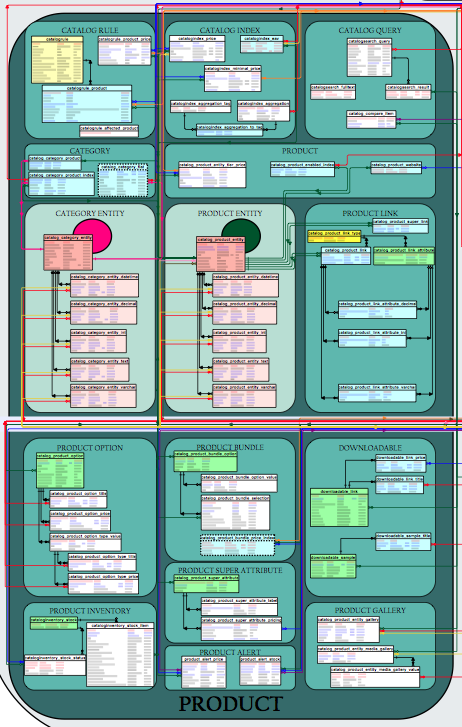
\includegraphics[width=0.3\textwidth]{figuras/cap2/magento_product_schema.png}
	\caption{Esquemas de un \itemCOM.}
	\label{cap:figure:catalog_magento}
\end{figure}

O realizar una sencilla búsqueda desde la \shell \mongodbNAME \javaScriptNAME  para obtener un objecto \jsonNAME como el \refsource{source:javascript:example_search_mongodb}.

Claramente en \refsource{source:javascript:example_search_mongodb} no hay representación completa de un \itemCOM, pero esto demuestra cuantas de estas \tablesDB triviales que existen en una representación relacional pueden prescindir en una representación \documentDB.

Para datos \objectOrientedPL, \textbf{los \documentsDB tienen mayor sentido}, tanto en concepto como rendimiento. Una representación \documentOriented de un dato de un \itemCOM se traduce a unas pocas entidades (un puñado de \collectionsDB vs. una docena de \tablesDB), mejor \performanceQA en consultas (sin \serverSideAS \joins), y estructuras que corresponden precisamente al \itemCOM. \textbf{Ya no existe la necesidad} de diseñar un \masterSchema que pueda considerar a cada tipo de \itemCOM concebible.

\catalogManagementCOM es esencialmente \contentManagementCOM, \textbf{un campo en donde \mongodbNAME sobresale}.

\subsubsection{\shoppingCarts y \ordersCommerce}

Permitir que un \shoppingCarts sea simplemente una orden en un estado  \cartCOM, el modelo de \shoppingCarts y las ordenes en \mongodbNAME se tornan muy sencillas. Un ejemplo de esto se puede observar en  \refsource{source:javascript:example_schema_order}.

Notar que es posible presentar los pedidos como un \arrayPL de \itemsCOM. Como es usual con \documentsDB, esto hace el despliegue del \shoppingCart mas sencillo, dado que no hay \joins envueltos. Pero esto también resuelve el problema del versionamiento de \itemsCOM. Usualmente es necesario tener el estado de un \itemCOM cuando este es comprado. Esto puede ser logrado en una \rdbms estableciendo un vínculo a versiones particulares de un \itemCOM. Aquí, sin embargo, simplemente se almacenó el estado de un \itemCOM dentro de la misma \orderCommerce.

\subsubsection{Consultando \ordersCommerce}

Dado que \mongodbNAME soporta consultas dinámicas y \secIndexingDB , las consultas para las \ordersCommerce son automáticas. Es posible, por ejemplo, definir un \indexDB en un \itemCOM \sku, lo que permite consultas eficientes en todas las ordenes para un \itemCOM dado. En  \refsource{source:javascript:example_querying_orders_mongodb} se observa un ejemplo.

Con \mongodbNAME, es posible realizar consultas en atributos arbitrarios, de esa manera, cualquier consulta en la \collectionDB \ordersCommerce es posible. Y para consultas comunes, es posible definir \indexesDB para una mejor eficiencia.

\subsubsection{\aggregationDB}

Claramente, \aggregationDB también es necesario. Se desea reportar \ordersCommerce de diferentes maneras, y para ese propósito, \mapReduce esta disponible. A modo de ejemplo, \refsource{source:javascript:example_aggregation_mongodb} tiene comando \mapReduce que \aggregatesDB el total de \ordersCommerce por \zipCode.

\subsubsection{\updating \ordersCommerce}

\subsubsection*{Incrementando Calidad}

Una manera de ajustar la cantidad es usando un \positionOperatorDB, el cual permite aplicar \atomicOperationsDB, a un único objeto dentro de un \arrayPL. \refsource{source:javascript:example_incrementing_quality_mongodb} muestra como cambiar el número de álbumes que se están ordenando.

 
\subsubsection*{\adding y \removing \itemsCOM}

Igualmente, \atomicOperationsDB resuelven el problema de agregar y remover \itemCOM desde el \cartCOM. \refsource{source:javascript:example_push_operator_mongodb} ejemplifica el uso de \pushOperatorDB \atomicOperatorDB para agregar un \itemCOM al \cartCOM.


Al ajustar la cantidad y el cambio de los mismos \itemsCOM en el \cartCOM, es necesario actualizar el total de la orden. Notar el uso del operador \incOperatorDB para manejar esto.

\subsubsection{\inventoryCommerce}

No todos los sitios \ecommerceCOM necesitan manejar el inventario. Pero para aquellos que si lo hacen, \mongodbNAME funciona a la altura de las circunstancias.

Una manera para manejar el inventario, es guardar un \documentDB separado por cada \physItem en la bodega. Así, por ejemplo, si la bodega tiene veinte copias del álbum Coltrane, se traduce en veinte \documentsDB distintos en \inventoryCommerce \collectionDB. Cada \documentDB tiene una estructura como lo muestra \refsource{source:javascript:example_document_inventory_mongodb}.


Cuando un usuario intenta agregar un \itemCOM al \cartCOM, un comando \findAndModifyOperatorDB puede ser facilitado para automáticamente marcar el \itemCOM en \inCart, asociando el \itemCOM con una \orderCommerce dada, y estableciendo un tiempo de espiración. \refsource{source:javascript:example_add_inventory_expiartion_mongodb}.



Si se obtiene un \itemBackDB desde la operación \findAndModifyOperatorDB, se sabe que tenemos un único \lockDB en el \itemCOM, y es posible guardarlo en el \cartCOM. Cuando el usuario desea realizar el \checkoutCOM, el estado del \itemCOM puede cambiar a \purchasedCOM, o cualquiera sea el caso de la llamada.

Mientras, se pueda ejecutar un \scriptPL en \backgroundPL que libere el inventario del \cartCOM que no ha sido \purchasedCOM en la ventana de quince minutos. La actualización es trivial y se observa en \refsource{source:javascript:example_add_script_background_mongodb}.


\subsubsection{\transactionsDB, \consistencyDB y \durabilityDB}

Muchos argumentos impuestos contra \nosqlNAME en \ecommerceCOM se centran en \transactionsDB, \consistencyDB, y \durabilityDB. En relación a esto se mencionan algunos puntos.

En relación a \transactionsDB, ciertamente \mongodbNAME no soporta el tipo \multiObjectDB; sin embargo, soporta \atomicOperationsDB sobre \documentsDB individuales. y esto combinado con el modelo \documentOriented recién descrito, y creatividad, es suficiente para muchos problemas \ecommerceCOM. Ciertamente, si se necesita \debitOneAccount y \creditAnother en la misma operación, ó si se desea \rollbackDB, sera necesario \fullFledgedTransDB. No obstante, \transactionalityDB provista por \mongodbNAME debería ser suficiente en la mayoría de los casos, si no en todos, para operaciones \ecommerceCOM.

Si la preocupación esta sobre \consistencyDB y \durabilityDB, operaciones escritas en \mongodbNAME pueden ser realizadas \consistencyDB sobre conexiones. Además, \mongodbNAME 1.5 soporta \nearRealTimeReplicationDB, así que es posible asegurarse que una operación ha sido \replicatedDB antes de retornar.

\subsubsection{\scalabilityQA}
La manera mas sencilla para \scale la mayoría de las \dataBasesDB, es \upgradingPC el \hardwarePC. Si la aplicación esta corriendo en un único nodo, es usualmente posible agregar una combinación de \diskPC \iopsPC, \memoryPC, y \cpuPC para eliminar los cuello de botella de la \dataBaseDB. La técnica de mejorar el \hardwarePC de un solo node para escalar se conoce como \verticalScalingDB o \scalingUpDB(\refFigura{figure:figure_scale_up}). \verticalScalingDB tiene la ventaja de ser simple, seguro, y \textit{costo-efectividad} hasta un cierto punto. Si se esta ejecutando sobre un \hardwarePC virtualizado( tal como \amazonEcdosNAME), entonces puedes encontrar que una instancia lo suficientemente larga no esta disponible. Si estas ejecutando sobre \physHardwarePC, habrá un punto donde el costo de un \serverAS mas poderoso se vuelve prohibitivo.

\begin{figure}[h!]
	\centering
	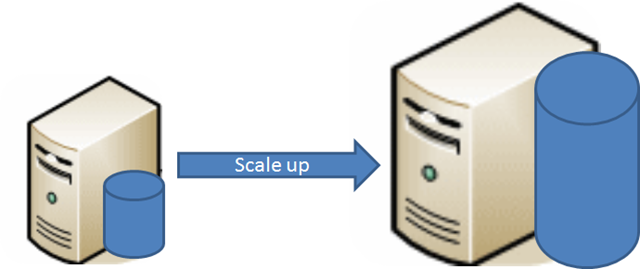
\includegraphics[width=0.5\textwidth]{figuras/cap2/scale_up.png}
	\caption{\verticalScalingDB ó \scalingUpDB }
	\label{figure:figure_scale_up}
\end{figure}

Entonces tiene sentido  considerar \horizontalScalingDB o \scalingOutDB(\refFigura{figure:figure_scale_out}). En lugar de reforzar un único nodo, \horizontalScalingDB significa distribuir la base de datos sobre múltiples máquinas. Dado que la arquitectura \horizontallyScaledDB puede utilizar \commodityHardwarePC, el costo de \hostingDB el total de los datos puede ser reducido significativamente. Incluso, la distribución  de los datos sobre máquinas mitiga las consecuencias de fallo. Las maquinas inevitablemente fallaran de algún momento a otro. En el caso de \verticalScalingDB , si la máquina falla, entonces es necesario tratar con una falla en un máquina de la cual la mayoría del sistema depende. Podría no considerarse un tema si una copia de los datos existe en un \replicatedSlaveDB, pero aun esta el caso en que solo un único \serverAS es necesario para bajar el sistema completo. En contraste con el fallo dentro de una arquitectura \horizontallyScaledDB. Esto podría ser menos catastrófico dado que una sola máquina representa un porcentaje menor del sistema completo.

\begin{figure}[h!]
	\centering
	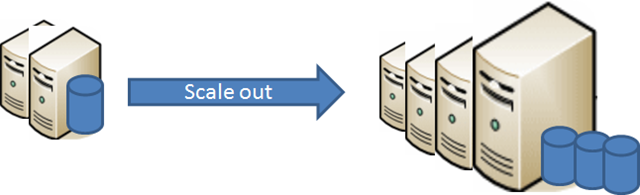
\includegraphics[width=0.5\textwidth]{figuras/cap2/scale_out.png}
	\caption{\horizontalScalingDB ó \scalingOutDB }
	\label{figure:figure_scale_out}
\end{figure}

\subsubsection{Conclusión}

Es cierto que la mayoría de las bases de datos \nosqlNAME no fueron construidas considerando \ecommerceCOM. Las bases de datos que carecen modelos de datos enriquecidos, consultas dinámicas, y la noción de \transactionalityDB no puede esperarse que compitan en el espacio de \ecommerceCOM, entonces no es comprensible que no se considere \mongodbNAME tampoco.

Pero para las partes en donde el sitio \ecommerceCOM comprende el manejo de contenido, \mongodbNAME es claro vencedor. E incluso para más componentes \transactionalDB del sistema, \mongodbNAME tiene características que hacen de la posibilidad de correr un sistema completo de \ecommerceCOM una realidad. Si bien es cierto que esto solo corresponde a un \sketchCPT, este permite obtener una noción de que \textbf{\documentsDB \dataBaseDB lo hace bien}.


\section{\nodejsNAME}\label{cap:section:nodejs}

%La craciente popularidad de JavaScript a traiado consigo una gran cantidad de cambios, y la manera en la cual los desarrolladores afrontan el desarrollo \textit{web} es dramaticamente distinto. Las cosas que se pueden hacer en la \textit{web} estos dias con JavaScript Corriendo en el servidor, de la misma manera como en el browser, era dificilmente imaginable hasta hace unos años atras, o fuimos encaptulados dentro de ambientes de \textit{sandbox} como Flash o Java Applets.
%JavaScript’s rising popularity has brought with it a lot of changes, and the face of web development today is dramatically different. The things that we can do on the web nowadays with JavaScript running on the server, as well as in the browser, were hard to imagine just several years ago, or were encapsulated within sandboxed environments like Flash or Java Applets.

%Before digging into Node.js, you might want to read up on the benefits of using JavaScript across the stack which unifies the language and data format (JSON), allowing you to optimally reuse developer resources. As this is more a benefit of JavaScript than Node.js specifically, we won’t discuss it much here. But it’s a key advantage to incorporating Node in your stack.

%As Wikipedia states: “Node.js is a packaged compilation of Google’s V8 JavaScript engine, the libuv platform abstraction layer, and a core library, which is itself primarily written in JavaScript.” Beyond that, it’s worth noting that Ryan Dahl, the creator of Node.js, was aiming to create real-time websites with push capability, “inspired by applications like Gmail”. In Node.js, he gave developers a tool for working in the non-blocking, event-driven I/O paradigm.

%After over 20 years of stateless-web based on the stateless request-response paradigm, we finally have web applications with real-time, two-way connections.

En una frase: \nodejsNAME brilla en aplicaciones \webINT \realTimeINT utilizando tecnología \pushINT sobre \websocketsINT. ¿Qué es tan revolucionario en relación a esto? Después de 20 años de \statelessWebINT en el paradigma \requestResponseINT finalmente existen aplicaciones \webINT \realTimeINT, conexiones \twoWayINT, donde \clientAS y \serverAS pueden iniciar la comunicación, permitiendo intercambiar datos libremente. Esto es un contraste enorme al paradigma típico de \webResponseINT, donde el \clientAS siempre iniciaba la comunicación. Adicionalmente, está todo basado en \openWebStackINT (\htmlNAME, \cssNAME y \javaScriptNAME )corriendo sobre el \standarPortINT 80.
%In one sentence: Node.js shines in real-time web applications employing push technology over websockets. What is so revolutionary about that? Well, after over 20 years of stateless-web based on the stateless request-response paradigm, we finally have web applications with real-time, two-way connections, where both the client and server can initiate communication, allowing them to exchange data freely. This is in stark contrast to the typical web response paradigm, where the client always initiates communication. Additionally, it’s all based on the open web stack (HTML, CSS and JS) running over the standard port 80.

Se puede discutir sobre que estas características existían hace años a través de \flashNAME y \javaAppletsINT, pero en realidad, esos fueron \sandboxedEnvPL utilizando la \webINT como un protocolo de transporte para entregar al \clientAS. Además, ellos corrían aislados y generalmente sobre \nonStandardPortsINT, los cuales podrían requerir permisos extras.
%One might argue that we’ve had this for years in the form of Flash and Java Applets—but in reality, those were just sandboxed environments using the web as a transport protocol to be delivered to the client. Plus, they were run in isolation and often operated over non-standard ports, which may have required extra permissions and such.

Con todas esta ventajas, \nodejsNAME ahora juega un role crítico en el \stackAS de tecnología de las principales compañías \highProfileCPT \cite{online_nodejs_highprofilecompanies} \textbf{las cuales dependen de sus beneficios únicos}.
%With all of its advantages, Node.js now plays a critical role in the technology stack of many high-profile companies who depend on its unique benefits.

%In this post, I’ll discuss not only how these advantages are accomplished, but also why you might want to use Node.js—and why not—using some of the classic web application models as examples.

%How Does It Work?

La principal idea de \nodejsNAME : usar \nonbloking, \eventdrivenPL \inputOutput para permanecer liviano y eficiente para enfrentar aplicaciones \dataintensive \realTimeINT que corren a través de dispositivos distribuidos.
%The main idea of Node.js: use non-blocking, event-driven I/O to remain lightweight and efficient in the face of data-intensive real-time applications that run across distributed devices.

%That’s a mouthful.

Lo que esto realmente significa es que \nodejsNAME no es una plataforma \panaceaCPT que dominara el mundo \webINT \developmentPC. \textbf{En lugar de eso, es una plataforma que llena una necesidad particular}. Esto es absolutamente esencial. Definitivamente no se deseara utilizar \nodejsNAME para operaciones \cpuIntensivePC; de hecho, utilizando esto para \heavyComputationPC anulará prácticamente todas sus ventajas. Donde \nodejsNAME realmente brilla es construyendo aplicaciones \scalableQA  \networkINT rápidamente, ya que es capaz de manejar un gran número de conexiones simultaneas con un alto rendimiento, lo que equivale a una \highScalabilityDB.
%What it really means is that Node.js is not a silver-bullet new platform that will dominate the web development world. Instead, it’s a platform that fills a particular need. And understanding this is absolutely essential. You definitely don’t want to use Node.js for CPU-intensive operations; in fact, using it for heavy computation will annul nearly all of its advantages. Where Node really shines is in building fast, scalable network applications, as it’s capable of handling a huge number of simultaneous connections with high throughput, which equates to high scalability.

Como trabaja \underTheHoodCPT es muy interesante. Comparado con la técnica tradicional \webServingINT donde cada conexión (\requestINT) engendra un nuevo \threadPL, ocupando memoria \memoryRamPC del sistema y, eventualmente \maxingOutCPT la cantidad de \memoryRamPC disponible, \nodejsNAME opera en un \singleThreadPL, usando llamadas \nonbloking \inputOutput, permitiendo el apoyo de decenas de miles de conexiones concurrentes (retenidas en el \eventloopCPT). \refFigura{figure:diagram_traditional_vs_nodejs_server_thread}.
%How it works under-the-hood is pretty interesting. Compared to traditional web-serving techniques where each connection (request) spawns a new thread, taking up system RAM and eventually maxing-out at the amount of RAM available, Node.js operates on a single-thread, using non-blocking I/O calls, allowing it to support tens of thousands of concurrent connections (held in the event loop).


\begin{figure}[h!]
	\centering
	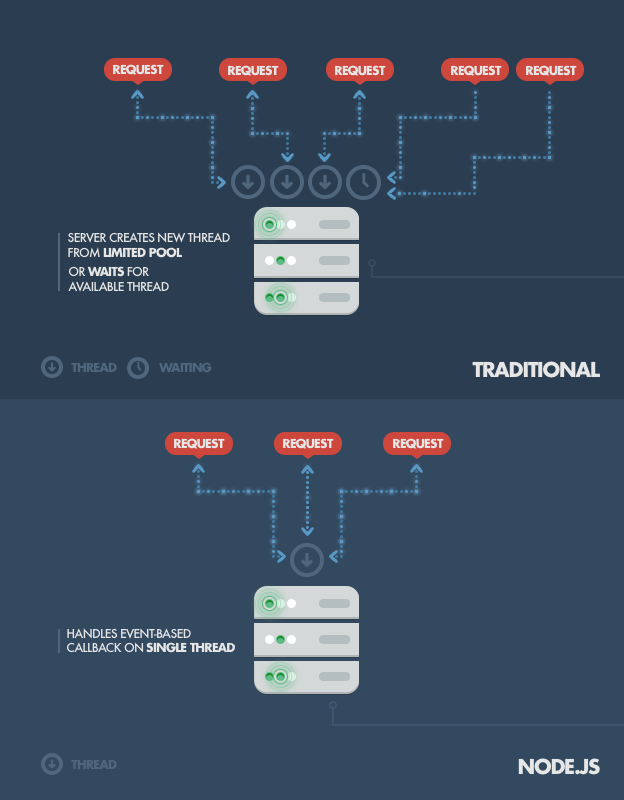
\includegraphics[width=0.5\textwidth]{figuras/cap2/diagram_traditional_vs_node_serverthread.png}
	\caption{Diagrama de Técnica tradicional vs. \nodejsNAME \serverAS \threadPL}
	\label{figure:diagram_traditional_vs_nodejs_server_thread}
\end{figure}



Un cálculo rápido: asumiendo que cada \threadPL potencialmente tiene asignado 2 MB de memoria con ella, corriendo en un sistema con 8 GB de \memoryRamPC nos coloca en un teórico máximo de 4000 conexiones concurrentes, además del costo por cambio de contexto entre \threadsPL. Ese es el escenario el cual típicamente se encuentran técnicas tradicionales de \webServingINT. Evitando todo eso, \nodejsNAME logra niveles de \scalabilityQA sobre 1M de conexiones concurrentes (como \proofConceptCPT).
%A quick calculation: assuming that each thread potentially has an accompanying 2 MB of memory with it, running on a system with 8 GB of RAM puts us at a theoretical maximum of 4000 concurrent connections, plus the cost of context-switching between threads. That’s the scenario you typically deal with in traditional web-serving techniques. By avoiding all that, Node.js achieves scalability levels of over 1M concurrent connections (as a proof-of-concept).

Hay, por supuesto, la cuestión de compartir un solo \threadPL entre todos los \requestINT de \clientsAS, y es una potencial trampa de escribir aplicaciones \nodejsNAME. Primeramente, \heavyComputationPC puede asfixiar el único \threadPL de \nodejsNAME y causar problemas en todos los clientes como \incommingRequestINT podrían ser bloqueados hasta que dicho \computationPC sea completado. En segundo lugar, desarrolladores necesitan ser realmente cuidadosos en no permitir que una excepción \bubblingUpPL al \coreAS del \eventloopCPT de \nodejsNAME, el cual puede causar que la instancia \nodejsNAME termine (efectivamente \crashingPC el programa).
%There is, of course, the question of sharing a single thread between all clients requests, and it is a potential pitfall of writing Node.js applications. Firstly, heavy computation could choke up Node’s single thread and cause problems for all clients (more on this later) as incoming requests would be blocked until said computation was completed. Secondly, developers need to be really careful not to allow an exception bubbling up to the core (topmost) Node.js event loop, which will cause the Node.js instance to terminate (effectively crashing the program).

La técnica utilizada para evitar excepciones \bubblingUpSurfacePL es pasando el error de regreso al \callerAS como parámetro de \callbackPL (en lugar de lanzarlos, como en otros ambientes). Incluso si alguna excepción no controlada conduce a \bubblingUpPL, hay múltiples paradigmas y herramientas disponibles para monitorear el proceso \nodejsNAME y realizar lo necesario para recuperarse de una \crashedInstancePL (aunque no este disponible para recuperar sesiones de usuarios), siendo el más común el módulo \moduleForeverNAME \cite{online_github_nodejitsu_forever}.
%The technique used to avoid exceptions bubbling up to the surface is passing errors back to the caller as callback parameters (instead of throwing them, like in other environments). Even if some unhandled exception manages to bubble up, there are mutiple paradigms and tools available to monitor the Node process and perform the necessary recovery of a crashed instance (although you won’t be able to recover users’ sessions), the most common being the Forever module, or a different approach with external system tools upstart and monit.

%NPM: The Node Package Manager

%When discussing Node.js, one thing that definitely should not be omitted is built-in support for package management using the NPM tool that comes by default with every Node.js installation. The idea of NPM modules is quite similar to that of Ruby Gems: a set of publicly available, reusable components, available through easy installation via an online repository, with version and dependency management.

%A full list of packaged modules can be found on the NPM website https://npmjs.org/ , or accessed using the NPM CLI tool that automatically gets installed with Node.js. The module ecosystem is open to all, and anyone can publish their own module that will be listed in the NPM repository. A brief introduction to NPM (a bit old, but still valid) can be found at http://howtonode.org/introduction-to-npm.

%Some of the most popular NPM modules today are:

%express - Express.js, a Sinatra-inspired web development framework for Node.js, and the de-facto standard for the majority of Node.js applications out there today.
%connect - Connect is an extensible HTTP server framework for Node.js, providing a collection of high performance “plugins” known as middleware; serves as a base foundation for Express.

%socket.io and sockjs - Server-side component of the two most common websockets components out there today.

%Jade - One of the popular templating engines, inspired by HAML, a default in Express.js.

%mongo and mongojs - MongoDB wrappers to provide the API for MongoDB object databases in Node.js.

%redis - Redis client library.
%coffee-script - CoffeeScript compiler that allows developers to write their Node.js programs using Coffee.
%underscore (lodash, lazy) - The most popular utility library in JavaScript, packaged to be used with Node.js, as well as its two counterparts, which promise better performance by taking a slightly different implementation approach.
%forever - Probably the most common utility for ensuring that a given node script runs continuously. Keeps your Node.js process up in production in the face of any unexpected failures.
%The list goes on. There are tons of really useful packages out there, available to all (no offense to those that I’ve omitted here).

%Examples of Where Node.js Should Be Used


%Where Node.js Can Be Used

%SERVER-SIDE WEB APPLICATIONS

%Node.js with Express.js can also be used to create classic web applications on the server-side. However, while possible, this request-response paradigm in which Node.js would be carrying around rendered HTML is not the most typical use-case. There are arguments to be made for and against this approach. Here are some facts to consider:

%Pros:

%If your application doesn’t have any CPU intensive computation, you can build it in Javascript top-to-bottom, even down to the database level if you use JSON storage Object DB like MongoDB. This eases development (including hiring) significantly.
%Crawlers receive a fully-rendered HTML response, which is far more SEO-friendly than, say, a Single Page Application or a websockets app run on top of Node.js.
%Cons:

%Any CPU intensive computation will block Node.js responsiveness, so a threaded platform is a better approach. Alternatively, you could try scaling out the computation [*].
%Using Node.js with a relational database is still quite a pain (see below for more detail). Do yourself a favour and pick up any other environment like Rails, Django, or ASP.Net MVC if you’re trying to perform relational operations.
%[*] An alternative to these CPU intensive computations is to create a highly scalable MQ-backed environment with back-end processing to keep Node as a front-facing ‘clerk’ to handle client requests asynchronously.
%Where Node.js Shouldn’t Be Used
%
%SERVER-SIDE WEB APPLICATION W/ A RELATIONAL DB BEHIND
%
%Comparing Node.js with Express.js against Ruby on Rails, for example, there is a clean decision in favour of the latter when it comes to relational data access.
%
%Relational DB tools for Node.js are still in their early stages; they’re rather immature and not as pleasant to work with. On the other hand, Rails automagically provides data access setup right out of the box together with DB schema migrations support tools and other Gems (pun intended). Rails and its peer frameworks have mature and proven Active Record or Data Mapper data access layer implementations, which you’ll sorely miss if you try to replicate them in pure JavaScript.[*]
%
%Still, if you’re really inclined to remain JS all-the-way (and ready to pull out some of your hair), keep an eye on Sequelize and Node ORM2—both are still immature, but they may eventually catch up.
%
%[*] It’s possible and not uncommon to use Node solely as a front-end, while keeping your Rails back-end and its easy-access to a relational DB.
%HEAVY SERVER-SIDE COMPUTATION/PROCESSING
%
%When it comes to heavy computation, Node.js is not the best platform around. No, you definitely don’t want to build a Fibonacci computation server in Node.js. In general, any CPU intensive operation annuls all the throughput benefits Node offers with its event-driven, non-blocking I/O model because any incoming requests will be blocked while the thread is occupied with your number-crunching.
%
%As stated previously, Node.js is single-threaded and uses only a single CPU core. When it comes to adding concurrency on a multi-core server, there is some work being done by the Node core team in the form of a cluster module [ref: http://nodejs.org/api/cluster.html]. You can also run several Node.js server instances pretty easily behind a reverse proxy via nginx.
%
%With clustering, you should still offload all heavy computation to background processes written in a more appropriate environment for that, and having them communicate via a message queue server like RabbitMQ.
%
%Even though your background processing might be run on the same server initially, such an approach has the potential for very high scalability. Those background processing services could be easily distributed out to separate worker servers without the need to configure the loads of front-facing web servers.
%
%Of course, you’d use the same approach on other platforms too, but with Node.js you get that high reqs/sec throughput we’ve talked about, as each request is a small task handled very quickly and efficiently.
%
%Conclusion
%
%We’ve discussed Node.js from theory to practice, beginning with its goals and ambitions, and ending with its sweet spots and pitfalls. When people run into problems with Node, it almost always boils down to the fact that blocking operations are the root of all evil—99% of Node misuses come as a direct consequence.
%
%In Node, blocking operations are the root of all evil—99% of Node misuses come as a direct consequence.
%
%Remember: Node.js was never created to solve the compute scaling problem. It was created to solve the I/O scaling problem, which it does really well.

%Why use Node.js? If your use case does not contain CPU intensive operations nor access any blocking resources, you can exploit the benefits of Node.js and enjoy fast and scalable network applications. Welcome to the real-time web.

\subsection{Desempeño de Node.js frente a sus competidores}
	A continuación se realizan comparaciones en el desempeño de la plataforma  con algunos de sus símiles mas conocidos los cuales corresponden a:
	
	\begin{itemize}
		\item Java
		\item Ruby
		\item PHP
	\end{itemize}

\subsubsection{\nodejsNAME vs \javaNAME \cite{online_nodejs_paypal}}



La primera adopción que hizo \paypalNAME con \nodejsNAME no fue una aplicación menor; esto fue su \accountOverviewPageINT y una de las mas \traffickedINT \appsINT en el \websiteINT. Ellos tomaron un gran riesgo, pero lo hicieron con la finalidad de determinar si realmente la nueva plataforma representaba una mejora con respecto al sistema actual.
%Our first adopter of node.js in production wasn’t a minor application; it was our account overview page and one of the most trafficked apps on the website. We decided to go big, but we also mitigated that risk by building the equivalent Java application in parallel. We knew how to deploy and scale Java applications, so if anything went wrong with the node.js app, we could fall back to the Java one. This provided the setting for some interesting data.

Una vez que la aplicación con \nodejsNAME logro las mismas funcionalidades que la aplicación actual, persivieron el siguiente resultado:

\begin{itemize}
\item Fue construida casi \textbf{el doble de rápido con menos personal}.
\item Escrito con un \textbf{33\% menos de lineas de código}.
\item Construida con \textbf{40\% menos de archivos}.
\end{itemize}

Por si solo, esta evidencia mostraba a los equipos desarrollar más rápido utilizando \javaScriptNAME.

\performanceQA fue un tópico interesante. Se pudo analizar 2 aplicaciones con exactamente las mismas funcionalidades: una con \frameworkPC \javaNAME interno basado en \javaSpringNAME y la otra construida en \krakenjsNAME usando \expressjsNAME, \dustjsNAME y otros códigos \openSourcePC.
%Performance is a fun and debatable topic. In our case, we had two applications with the exact same functionality and built by roughly the same teams: one on our internal Java framework based on Spring and the other built on kraken.js using express, dust.js and other open source code.

Se ejecutaron los test adecuados utilizando \hardwarePC de producción que probaran las rutas y recolectaran datos de rendimiento y tiempo de respuesta. Los resultados se aprecian en \refFigura{figure:java_benchmark_paypal}.
%We ran our test suite using production hardware that tested the routes and collected data on throughput and response time.

\begin{figure}[H]
	\centering
	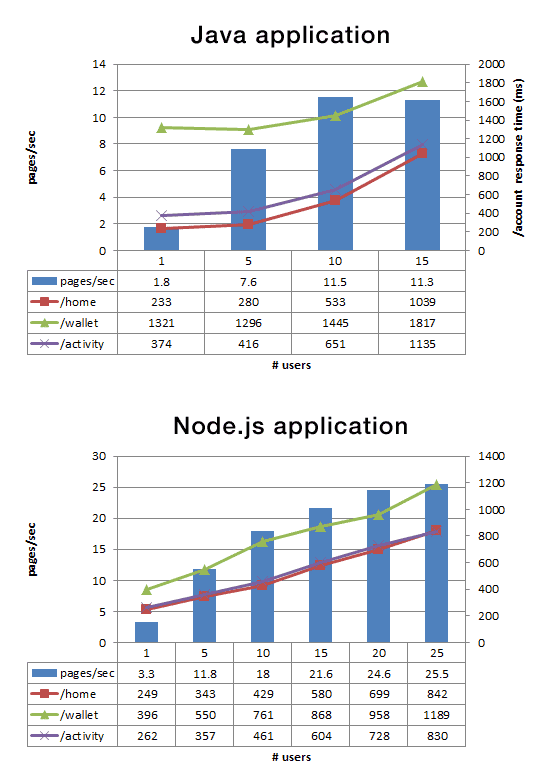
\includegraphics[width=0.6\textwidth]{figuras/cap2/java_nodejs_benchmark_paypal.png}
	\caption{\performanceQA de la aplicación en \javaNAME y \nodejsNAME}
	\label{figure:java_benchmark_paypal}
\end{figure}

Se observa que la aplicación utilizando \nodejsNAME tiene:
%You can see that the node.js application had:

\begin{itemize}
\item El doble de solicitudes por segundo vs. la aplicación \javaNAME. Esto es incluso más interesante porque los resultados iniciales de rendimiento estaban utilizando un solo núcleo para la aplicación \nodejsNAME, en comparación con cinco núcleos en \javaNAME. Esperan aumentar aun más esta brecha en el futuro.
%Double the requests per second vs. the Java application. This is even more interesting because our initial performance results were using a single core for the node.js application compared to five cores in Java. We expect to increase this divide further.
\item \textbf{Disminución en un 35\% en el tiempo promedio de respuesta} para la misma página. Esto resulto ser \textbf{200ms mas rápido} en el \serverAS. Algo que los usuarios definitivamente notan.
%35% decrease in the average response time for the same page. This resulted in the pages being served 200ms faster— something users will definitely notice.
\end{itemize}

%There’s a disclaimer attached to this data: this is with our frameworks and two of our applications. It’s just about as apples-to-apples a performance test as we could get between technologies, but your milage may vary. That said, we’re excited by what we’ve seen from node.js’ raw performance.

Mas ejemplos de \benchmarkQA pueden ser encontrados en\cite{online_nodejs_java_dzone}.


\subsubsection{\nodejsNAME vs \railsNAME \cite{online_nodejs_ruby_linkid}}

De acuerdo a un estudio que realizó \linkedInNAME en el cual evaluó tres posibles soluciones: \railsNAME/\eventMachineCPT; \pythonNAME/\twistedCPT y \nodejsNAME. Se determinaron los siguientes beneficios de parte de \nodejsNAME:
%LinkedIn evaluated three possible solutions: Rails/Event Machine, Python/Twisted, and Node.js. According to Prasad, Node.js was eventually chosen providing a number of benefits:

\begin{itemize}
	\item
		Mejor \performanceQA, \nodejsNAME alcanzando hasta 20 veces más rápido que \railsNAME en ciertos escenarios.
		%Better performance, Node.js being up to 20x faster than Rails for certain scenarios
	\item
		Usando solo 3 \serverAS en lugar de 30, dejando espacio para un crecimientos de 10 veces el tráfico.
		%Using only 3 servers instead of 30, leaving room for a 10x traffic growth
	\item
		Ingenieros \javaScriptNAME \frontEndAS pudieron ser utilizados para código \backendAS, y los dos equipos se transformaron en uno.
		%Front-end JavaScript engineers could be used for back-end code, and the two teams were actually merged into one

\end{itemize}


\subsubsection{\nodejsNAME vs \phpNAME \cite{online_nodejs_php_loadimpact}}

No es justo comparar \nodejsNAME con \phpNAME. Lo que realmente se compara es \nodejsNAME y \phpNAME + \apacheDosNAME ( u otro servidor \httpNAME ). Es este caso particular, las pruebas fueron realizadas usando \apacheDosNAME y \modPhpNAME, dado que es por lejos la configuración mas común. 
%So no, it’s not fair to say that we compare Node.js and PHP. What we really compare is Node.js and PHP+Apache2 (or any other http server). For this article, I’ve used Apache2 and mod_php since it’s by far the most common configuration. Some might say that I’d get much better results if I had used Nginx or Lighthttpd as the http server for PHP. That’s most likely very true, but at the end of the day, server side PHP depends on running in multiple separate processes. Regardless if we create those processes with mod_php or fastcgi or any other mechanism. So, I’m sticking with the standard server setup for PHP and I think that makes good sense.

\begin{figure}[H]
	\centering
	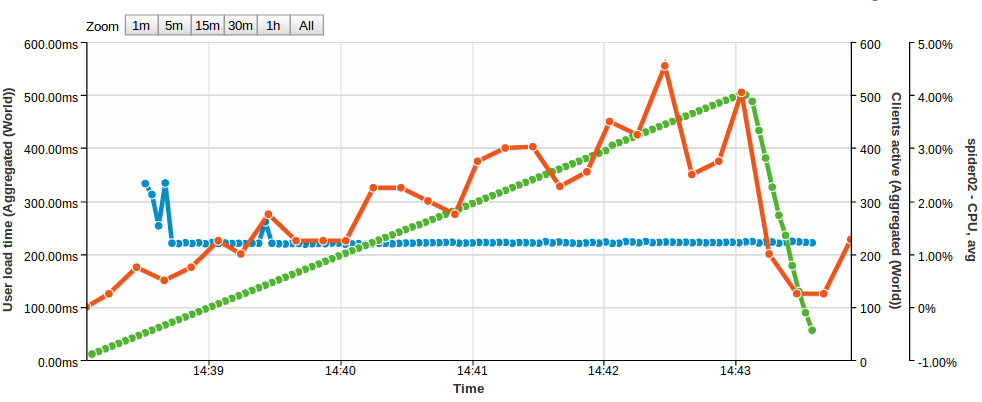
\includegraphics[width=0.6\textwidth]{figuras/cap2/node_benchmak_loadimpact.png}
	\caption{\performanceQA de la aplicación \nodejsNAME}
	\label{figure:node_benchmark_nodephp}
\end{figure}

El gráfico de \refFigura{figure:node_benchmark_nodephp} muestra lo que sucede cuando se carga el test en el \serverAS utilizando \nodejsNAME. La respuesta de tiempo (azul) es mucho mas constante durante todo el test. 

%The first graph here shows what happens when we load test the Node.js server. The response time (blue) is pretty much constant all through the test. My back of a napkin analysis of the initial outliers is that they have to do with a cold MySQL cache. Now, have a look at the results from the PHP test:


\begin{figure}[H]
	\centering
	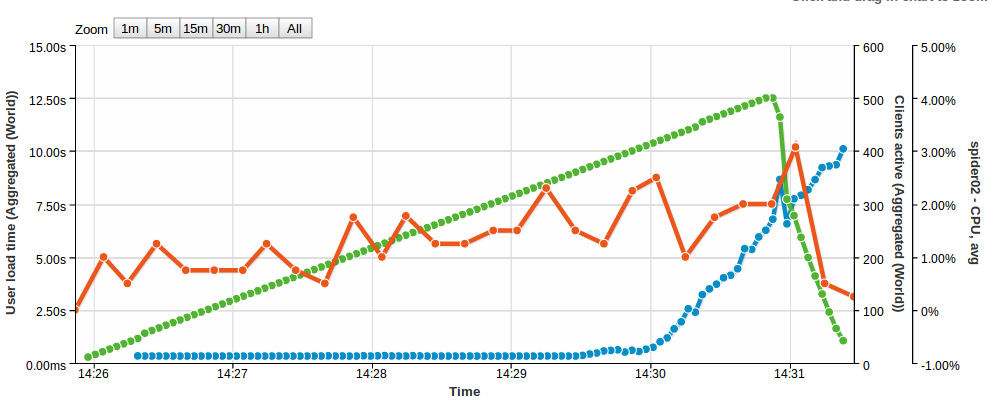
\includegraphics[width=0.6\textwidth]{figuras/cap2/phpapache_benchmak_loadimpact.png}
	\caption{\performanceQA de la aplicación en \phpApacheNAME}
	\label{figure:php_benchmark_nodephp}
\end{figure}

Muy diferente los resultados para el caso de \phpNAME(\refFigura{figure:php_benchmark_nodephp}). No es sencillo observar que sucede, pero las lineas azules están inicialmente estables a 320ms hasta cerca de 340 usuarios activos simultáneos. Después de eso, se observa un pequeño incremento en el tiempo de respuesta pero después de agregar mas usuarios activos simultáneos, el tiempo de respuesta se dispara por completo. 
%Quite different results. It’s not easy to see on this screen shot, but the blue lines is initially stable at 320 ms response time up to about 340 active concurrent users. After that, we first see a small increase in response time but after additional active concurrent users are added, the response time eventually goes through the roof completely.

¿ Qué problema tiene \phpApacheNAME?
%So what’s wrong with PHP/Apache?

La diferencia no es de sorprender. Esto es producto de la diferencia de arquitectura entre ambas soluciones.
%Ok, so what we’re looking at is not very surprising, it’s the difference in architecture between the two solutions. Let’s think about what goes on in each case.

Cuando \apacheDosNAME sirve a una pagina \phpNAME, este deja la ejecución \phpNAME a un \childProcessPC específico. Ese \childProcessPC puede solo manejar una solicitud \phpNAME al mismo tiempo, así que si hay más solicitudes, las otras deben esperar. En el \serverAS hay un máximo de 256 \clientsAS (\maxClientsDB) configurados vs 150 que vienen por defecto. Incluso si es posible aumentar el \maxClientsDB hasta mas allá de 256, habrá problemas con la memoria interna(\memoryRamPC), Al final, se necesita encontrar el balance correcto entre el máximo número de solicitudes simultaneas y los recursos disponibles del \serverAS.
%When Apache2 serves up the PHP page it leaves the PHP execution to a specific child process. That child process can only handle one PHP request at a time so if there are more requests than than, the others have to wait. On this server, there’s a maximum of 256 clients (MaxClients) configured vs 150 that comes standard. Even if it’s possible to increase MaxClients to well beyond 256, that will in turn give you a problem with internal memory (RAM). At the end, you need to find the correct balance between max nr of concurrent requests and available server resources.

Pero para \nodejsNAME, es sencillo. Después de todo, cada solicitud es cerca de 30\% más rápido que \phpNAME, así que en \performanceQA, el cual es una configuración extremadamente básica, \nodejsNAME es mas rápido. Además, en\nodejsNAME Todo esta en un solo proceso en el \serverAS. Un proceso manejando una solicitud activa. Así que no existe una comunicación interna de procesos entre diferentes instancias y el proceso madre. Incluso, pos solicitud, \nodejsNAME es mucho mas eficiente. \phpApacheNAME necesita muchísimo \phpNAME y sobrecarga de procesos por cada \workerClientINT concurrente mientras \nodejsNAME compartirá la mayoría de su memoria entre las solicitudes.
%But for Node, it’s easier. First of all, in the calm territory, each request is about 30% faster than for PHP, so in pure performance in this extremely basic setup, Node is quicker. Also going for Node is the fact that everything is in one single process on the server. One process with one active request handling thread. So thre’s no inter process communication between different instances and the ‘mother’ process. Also, per request, Node is much more memory efficient. PHP/Apache needs to have a lot of php and process overhead per concurrent worker/client while Node will share most of it’s memory between the requests.

%Also note that in both these tests, CPU load was never a problem. Even if CPU loads varies with concurrent users in both tests it stays below 5% (and yes, I did not just rely on the graph, I checked it on the server as well). (I’ll write a follow up on this article at some point when I can include server memory usage as well). So we haven’t loaded this server into oblivion in any way, we’ve just loaded it hard enough for the PHP/Aapache architecture to start showing some of it’s problems.

Más ejemplos de \benchmarkQA pueden ser encontrados en \cite{online_nodejs_java_appdynamics}.


%\subsubsection*{¿ Qué hace a Node.js mejor?}
%
%Node.js introduce al menos 2 nuevas características ( para una amplia audiencia ). Primero, la habilidad  de escribir código JavaScript en el lado del servidor. En teoría esto puede ser una ventaja dado que JavaScipt es mas importante que nunca en el lado del cliente y usando el mismo lenguaje en el servidor y en el navegador deberían haber muchísimos beneficios. 
%%Node.js introduces at least two new things (for a broader audience). First, the ability to write server side JavaScript code. In theory this could be an advantage since JavaScript is more important than ever on the client side and using the same language on server and browser would have many benefits. That’s at least quite cool.
%
%La otra cosa que introduce Node.js es que es completamente asíncrono y orientado al evento. Node.js esta basado en el supuesto que muchísimo código de computador realmente espera por I/O la mayoría del tiempo, como esperando por un archivo para ser escrito en el disco o por una solicitud MySQL para retornar \textit{data}. Para lograr eso, mas o menos cada función en Node.js es \textit{non-blocking}.
%%The other thing that makes Node.js different is that it’s completely asynchronous and event driven. Node is based on the realization that a lot of computer code actually just sits idle and wait for I/O most of the time, like waiting for a file to be written to disk or for a MySQL query to return data. To accomplish that, more or less every single function in Node.js is non-blocking.
%
%Cuando se solicita a nodo abrir un archivo, no se espera a que retorne. En lugar de eso, se le comunica a Node.js a que función se le entrega el resultado y continuar con otra ejecución. Esto conduce a una dramática diferencia  para estructurar el código con \textit{callback} anidados y funciones anónimas de clausura.  Terminaras con algo como esto:
%%When you ask for node to open a file, you don’t wait for it to return. Instead, you tell node what function to pass the results to and get on with executing other statements. This leads to a dramatically different way to structure your code with deeply nested callbacks and anonymous function and closures. You end up with something  like this:
%
%
%\medskip
%\begin{lstlisting}[caption= Ejemplo de anidación de funciones.]
%	doSomething(val, function(err,result){
%		doSomethingElse(result,function(err,res){
%			doAbra();
%			doKadabra(err, res, function() {
%				...
%				...
%			});
%		});
%	});
%\end{lstlisting}
%
%
%La cualidad que hace diferente a Node.js, es que no es necesario utilizar un servidor http(s) separado. Es completamente común poner Node.js detrás de un Nginx, pero eso no es estrictamente necesario. Así que el corazón de las aplicaciones \textit{web} típicas de Node.js  es la implementación de su servidor real.
%It’s quite easy to end up with very deep nesting that in my opinion sometimes affects code readability in a negative way. But compared to what gets said about PHP, that’s very mild critique. And.. oh! The third thing that is quite different is that in Node.js, you don’t have to use a separate http(s) server. It’s quite common to put Node.js behind a Nginx, but that’s not strictly needed. So the heart of a typical Node.js web application is the implementation of the actual web server.
%
%
%*****************************************************************************
%
%
%Hopefully, this shows the inherit differences in two different server technologies. One old trusted and one young and trending. Hopefully it’s apparent that your core technical choices will affect your server performance and in the end, how much load you can take. Designing for high load and high scalability begins early in the process, before the first line of code is ever written.
%
%And sure, in real life, there are numerous of tricks available to reduce the effects seen here. In real life, lots of Facebook still runs on PHP.

\subsection{\fullstackAS \javaScriptNAME}

La elección del uso de \nodejsNAME trae como consecuencia inmediata el uso de \javaScriptNAME en \serverSideAS. Hay una gran cantidad de ventajas al utilizar un único lenguaje a lo largo del \stackAS. Al programas con \javaScriptNAME existe la posibilidad de realizar mejoras de rendimiento tanto en el propio \softwarePC y en la productividad de los desarrolladores. Con \mongodbNAME, se puede guardar los \documentsDB en un formato \jsonLikeCPT, escribir consultas \jsonNAME en los servidores basados en \nodejsNAME, y similarmente pasar documentos \jsonNAME al \frontEndAS. \debuggingPL y la administración de la base de datos se vuelve una tarea muchísimo mas sencilla cuando los objetos guardados en la base de datos son esencialmente idénticos a los objetos que el cliente \javaScriptNAME ve. Incluso mejor, alguien trabajando en \clientSideAS puede fácilmente entender el código del \serverSideAS y las consultas a la \dataBaseDB; usando la misma sintaxis y objetos todo el proceso libera a los desarrolladores la consideración de varios conjuntos de buenas prácticas de lenguajes y reduce la barrera de entrada para la comprensión de su código base. Esto es especialmente importante en una \hackathonCPT: el equipo puede no tener mucha experiencia trabajando juntos, y con tan poco tiempo para integrar todas las piezas de su proyecto, cualquier detalle que haga el proceso de desarrollo más sencillo es oro.
%First of all, there are huge advantages to using a uniform language throughout your stack. My team uses a set of tools that we affectionately call the MEAN stack:­ MongoDB, ExpressJS, AngularJS, and Node.js. By coding with Javascript throughout, we are able to realize performance gains in both the software itself and in the productivity of our developers. With MongoDB, we can store our documents in a JSON-­like format, write JSON queries on our ExpressJS and NodeJS based server, and seamlessly pass JSON documents to our AngularJS frontend. Debugging and database administration become a lot easier when the objects stored in your database are essentially identical to the objects your client Javascript sees. Even better, somebody working on the client side can easily understand the server side code and database queries; using the same syntax and objects the whole way through frees you from having to consider multiple sets of language best practices and reduces the barrier to entry for understanding your codebase. This is especially important in a hackathon setting: the team may not have much experience working together, and with such little time to integrate all the pieces of your project, anything that makes the development process easier is gold.



\subsection{\nodejsNAME y \ecommerceCOM}

\ecommerceCOM es un excelente ejemplo de sistema que se puede ver totalmente beneficiado con el uso de \nodejsNAME en el lado del \serverAS. 

\begin{itemize}
	\item \textbf{\frontEndAS se movió desde el \serverSideAS al \clientSideAS ( al menos en \mobileINT )}. Una de las grandes consecuencias es que el \serverSideAS ya no es más \cpuBoundPC ahora es \memoryBoundPC e \ioBoundPC. \nodejsNAME es \eventdrivenPL, lo cual implica eficiencia en \ioBoundPC y es extremadamente eficiente en el uso de memoria.
	\item Permite velocidad de desarrollo y ejecución. En otras palabras iteraciones rápidas.
	%Ease of Development-Some problem, somewhere has a solution best written in Brainf*ck. But implementing that solution (in Brainfuck) will be nearly impossible to write, let alone read. It will cost you time and a tremendous amount of effort. In general, you should use languages and platform that make development easier, not harder for you (or anyone that might work on it later).
	\item \textbf{Comunidad}: Existe una activa comunidad la cual esta constantemente solucionando dudas, además de proporcionar módulos para resolver problemas conocidos.
	\item \textbf{Reutilizar código}: \serverSideAS y \clientSideAS usan el mismo lenguaje, permitiendo reutilización de componentes.
	\item \textbf{Optimiza el uso de recursos}: Los desarolladores de \clientSideAS pueden desarrollar en \serverSideAS, ya que son el mismo lenguaje.
	\item \textbf{\scalabilityQA}: Los sitios \webINT se encuentran en constante crecimiento. \scalabilityQA es una consecuencia de la eficiencia que tiene \nodejsNAME para \memoryBoundPC e \ioBoundPC
\end{itemize}

%+++++++++++++++++++++++++++++++++++++++++++++++++++++++++++++++++++++++
%
%
%Node no es la panacea para todo, tiene muchos issues con los cuales hay que lidiar, pero es probable una de las mejores soluciones que se pueden tomar(LinkedIn).
%
%***************************************************************************
%Kiran Prasad, Sr. Director, Mobile Engineering, LinkedIn
%
%Una pregunta interesante saber cuales son los problemas que te hicieron mirar hacia nodeJ(pregunta a KIRAN Prased)
%
%Cuando llegue a LinkedIN estabamos corriendo cosas en Ruby and Rails stack, una de las cosas que encontramos es que el FRONT-END se movio desde el server-side al client-side( al menos en mobile ). Ese gran shift cambio  las necesidades del front-end y el server-side.
%
%El server-side ya no es mas CPU Bound ahora es Memory Bound e I/O Bound
%
%Nodejs run de forma muy eficiente en I/O 
%
%Dio velocidad de desarrollo, de ejecución, iteraciónes mas rápidas 
%
%Este tipo de razones nos mostrarón la necesidad de I/O Bound necesitan ser I/O event
%Necesitaban eficiencia de memoria, y Node es super eficiente en ese sentido.
%La convinación de estos elementos  
%
%eficiencia en memoria
%
%
%
%***************************************************************************
%Sri Viswanath, SVP Engineering and Operations, Groupon
%
%
%
%Need low latency
%
%
%
%***************************************************************************
%Jigar Desai, Sr. Director, Platforms, eBay
%
%
%
%
%
%
%***************************************************************************
%Billy Scott, PayPal

%%%%%%%%%%%%%%%%%%%%%%%%%%%%%%%%%%%%%%%%%%%%%%%%%%%%%%%%%%%%%%%%%%%%%%%%%%%%%
%%%%%%%%%%%%%%%%%%%% 	    FUTURO APLICACIONES WEB  	 %%%%%%%%%%%%%%%%%%%%
%%%%%%%%%%%%%%%%%%%%%%%%%%%%%%%%%%%%%%%%%%%%%%%%%%%%%%%%%%%%%%%%%%%%%%%%%%%%%


%\section{Aplicaciones \webINT}\label{cap:estadoArte:section:web_app}
\section{\isomorphicAS \javaScriptNAME : el futuro de las aplicaciones \webINT}\label{cap:estadoArte:section:web_app}
Cuando se utiliza un \backendAS corriendo una aplicación \javaNAME, \phpNAME o \railsNAME, el proceso ocurre muy lejos del usuario. Los \clientsAS solicitan datos llamando una \uriNAME. En respuesta, la aplicación trae datos desde una \dataBaseDB, realiza algún procedimiento para crear \htmlNAME y envía los resultados al \clientAS. Mientras mayor sea el número de \clientsAS que realizan la misma solicitud, los mecanismos inteligentes de \caching pueden ser usados por el \serverAS. \sitesINT de noticias funcionan particularmente bien en este tipo de paradigma.
%When using a backend running a Java, PHP, or Rails application, processing takes place far away from the user. Clients request data by calling a URI. In response the application fetches data from a database, performs some processing to create HTML and sends the results to a client. The more clients request the same information, the more clever caching mechanisms can be used by the server. News sites work particularly well with this paradigm.

En un escenario en donde cada usuario realiza solicitudes para crear vistas altamente individualizadas, un único proceso de instancia rápidamente se convierte en un cuello de botella. Considerando a \facebook como un ejemplo: Dos personas nunca verán exactamente un mismo \facebookwall, esto es calculado individualmente para cada usuario. Esto agrega una gran cantidad de \stress en el servidor mientras el cliente está en su mayoría de tiempo \idle, esperando una respuesta.
%In a scenario where each user has the means to create highly individualized views a single processing instance can quickly become a bottle neck. Consider Facebook as an example: No two people will ever see the exact same wall, it needs to be computed for each user individually. That puts a lot of stress on the servers while clients idle most of the time, waiting for a response.

Cuando el poder de procesamiento de un cliente era relativamente limitado, este enfoque tenia sentido, pero en la actualidad un solo \smartphoneCPT tiene más poder de cómputo que muchos de los súper computadores en los primeros años de la \webINT. Los nuevos enfoques toman ventaja de ese poder y delegan la mayoría del proceso a los \clientsAS. \frontEndsAS inteligentes solicitan información al \serverAS y montan el \htmldomNAME en el \browserINT.
%When the processing power of clients was relatively limited this made perfect sense, but these days a single iPhone already has more computing power than most super computers in the early days of the web. Meteor takes advantage of that power and delegates most of the processing to the clients. Smart front-ends request data from the server and assemble the DOM only in the browser or mobile device (see Figure 1-4).

Este enfoque \clientcentric implica dos ventajas significativas:
%This client-centric approach brings two significant advantages:
\begin{itemize}
	\item Menos necesidad de transferencia de información entre el \serverAS y el \clientAS, lo que esencialmente se traduce como tiempos de respuesta mas rápidos.
%1. Less data needs to be transferred between server and client which essentially translates into quicker response times
	\item Existe una menor probabilidad de que el procesamiento sea bloqueado por otros usuarios debido a peticiones de duración prolongada, ya que la mayor parte del trabajo se realiza individualmente en cada \clientAS.
%2. Processing is less likely to be blocked by other users due to long-running requests, as most of the work is done on each individual client
\end{itemize}

La arquitectura \clientserver se basa en \statelessconnectionsINT. \clientsAS solicitan información una vez, el \serverAS responde y la conexión es cerrada nuevamente. Actualizaciones en otros clientes pueden suceder, a menos que explícitamente realiza una solicitud al \serverAS nuevamente, no verán actualizaciones. No existe un canal de \feedback del \serverAS al \clientAS para enviar actualizaciones de contenido.

Mover el proceso desde un solo \serverAS a múltiples \clientsAS envuelve moverse en dirección a una plataforma de cómputo distribuida. En tal situación, los datos deben ser enviados en ambas direcciones.

Después de muchos años de avance, se desarrollaron soluciones muy creativas que impulsaron a los \browsersINT a mejorar para mantenerse a la par. 
Actualmente la \webINT se ha transformado en una plataforma de aplicaciones \fullyfeatured, \runtimesCPT \javaScriptNAME rápidos y \standard \htmlfive que permite crear aplicaciones que antes eran solo posibles en plataformas nativas.

\subsection{\singlePageAppINT}

No pasó mucho tiempo hasta que los desarrolladores comenzaron a crear aplicaciones completas en el \browserINT utilizando las nuevas capacidades de \javaScriptNAME y \htmlfive para crear \singlePageAppINT. Una \spa es una aplicación \webINT completa, la cual solo tiene una página, que es usada como un contenedor para todas las páginas \webINT de la aplicación y utiliza \javaScriptNAME, \htmlfive y \cssNAME para todas las interacciones \frontEndsAS. En \spas no hay \posts completos de vuelta al \serverAS, no hay refrescos completos de una página \webINT, y no hay objetos embebidos. La principal diferencia con las aplicaciones \webINT tradicionales es la naturaleza de las \requests y \responsesINT que siguen al \requestINT \httpNAME inicial. Con \spa se utiliza \ajaxNAME para \requestINT datos y se obtiene un \responsesINT correspondiente a datos \jsonNAME. Una vez que la información es recibida por el \clientAS, este hará un \renderCPT parcial de \htmlNAME para representar los cambios. Incluso, moviéndonos de una página a otra en un \spa ocurre en \clientSideAS, lo que es diferente a lo que sucede en aplicaciones tradicionales y \ria.

Librerías como \backbonejsNAME \emberjsNAME, y \angularjsNAME usualmente son referidas como librerías \clientSideAS \mvcAS o \mvvmAS. La arquitectura típica \clientSideAS \mvcAS se ve similar a la \refFigura{figure:client_side_mvc}. 
%Libraries like Backbone.js, Ember.js, and Angular.js are often referred to as client-side MVC (Model-View-Controller) or MVVM (Model-View-ViewModel) libraries. The typical client-side MVC architecture looks something like this:

% GRAFICO CLIENT SIDE MVC 

%\begin{figure}[h!]
\begin{figure}[H]
	\centering
	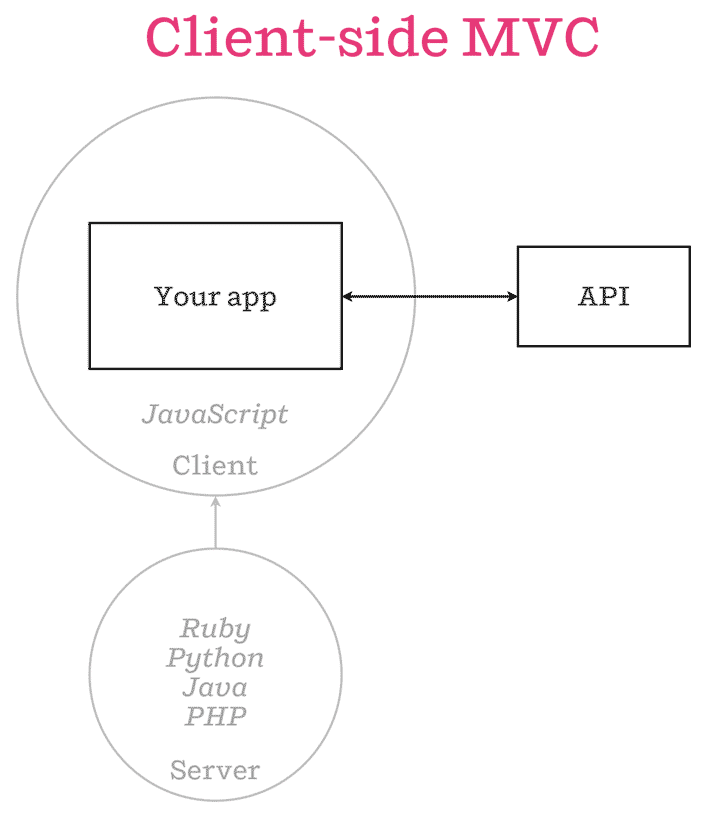
\includegraphics[width=0.5\textwidth]{figuras/estadoArte/isomorphic-client-side-mvc.png}

	\caption{\clientSideAS \mvcAS.}
	\label{figure:client_side_mvc}
\end{figure}

% Definition of circles
% \def\firstcircle{(0,0) circle (2)}
% \def\secondcircle{(0,-5) circle (1)}

% \def\firstrectangle{(-1.5,1) rectangle (1.5,-1)}

% \def\secondrectangle{(4,0.5) rectangle (6.5,-0.5)}

% \colorlet{circle edge}{blue!50}
% \colorlet{circle area}{blue!20}

% \tikzset{filled/.style={fill=circle area, draw=circle edge, thick},
%     outline/.style={draw=circle edge, thick}}

% \setlength{\parskip}{5mm}
% % Set A and B
% \begin{tikzpicture}
%     \begin{scope}
%         \clip \firstcircle;
%         \fill[filled] \secondcircle;
%     \end{scope}

%     \draw \firstrectangle node {$Aplicacion$};
%     \draw \secondrectangle node {$API$};

%     \draw[outline] \firstcircle node {$A$};
%     \draw[outline] \secondcircle node {$B$};
%     \node[anchor=south] at (current bounding box.north) {$A \cap B$};
% \end{tikzpicture}









% \newcommand{\mx}[1]{\mathbf{\bm{#1}}} % Matrix command
% \newcommand{\vc}[1]{\mathbf{\bm{#1}}} % Vector command

% % Define the layers to draw the diagram
% \pgfdeclarelayer{background}
% \pgfdeclarelayer{foreground}
% \pgfsetlayers{background,main,foreground}

% % Define block styles used later

% \tikzstyle{sensor}=[draw, fill=blue!20, text width=5em, 
%     text centered, minimum height=2.5em,drop shadow]
% \tikzstyle{ann} = [above, text width=5em, text centered]
% \tikzstyle{wa} = [sensor, text width=10em, fill=red!20, 
%     minimum height=6em, rounded corners, drop shadow]
% \tikzstyle{sc} = [sensor, text width=13em, fill=red!20, 
%     minimum height=10em, rounded corners, drop shadow]

% % Define distances for bordering
% \def\blockdist{2.3}
% \def\edgedist{2.5}

% \begin{tikzpicture}
%     \node (wa) [wa]  {System Combination};
%     \path (wa.west)+(-3.2,1.5) node (asr1) [sensor] {$ASR_1$};
%     \path (wa.west)+(-3.2,0.5) node (asr2)[sensor] {$ASR_2$};
%     \path (wa.west)+(-3.2,-1.0) node (dots)[ann] {$\vdots$}; 
%     \path (wa.west)+(-3.2,-2.0) node (asr3)[sensor] {$ASR_N$};    
   
%     \path (wa.east)+(\blockdist,0) node (vote) [sensor] {$\theta_0,\theta_1,...,\theta_M$\\Estimated Parameters};

%     \path [draw, ->] (asr1.east) -- node [above] {} 
%         (wa.160) ;
%     \path [draw, ->] (asr2.east) -- node [above] {} 
%         (wa.180);
%     \path [draw, ->] (asr3.east) -- node [above] {} 
%         (wa.200);
%     \path [draw, ->] (wa.east) -- node [above] {} 
%         (vote.west);

               
%     \path (wa.south) +(0,-\blockdist) node (asrs) {System Combination - Training};
  
%     \begin{pgfonlayer}{background}
%         \path (asr1.west |- asr1.north)+(-0.5,0.3) node (a) {};
%         \path (wa.south -| wa.east)+(+0.5,-0.3) node (b) {};
%         \path (vote.east |- asrs.east)+(+0.5,-0.5) node (c) {};
          
%         \path[fill=yellow!20,rounded corners, draw=black!50, dashed]
%             (a) rectangle (c);           
%         \path (asr1.north west)+(-0.2,0.2) node (a) {};
            
%     \end{pgfonlayer}
    
%     % Validation Layer is the same except that there are a set of nodes and links which are added
   

%     \path (wa.south)+(-2.0,-7.5) node (syscomb) [sc] {\textbf{System Combination \\Algorithm}\\Estimated Parameters\\from training};
%     \path (syscomb.west)+(-2.2,1.5) node (asrt1) [sensor] {$ASR_1$};
%     \path (syscomb.west)+(-2.2,0.5) node (asrt2)[sensor] {$ASR_2$};
%     \path (syscomb.west)+(-2.2,-1.0) node (dots)[ann] {$\vdots$}; 
%     \path (syscomb.west)+(-2.2,-2.0) node (asrt3)[sensor] {$ASR_N$};    

%     \path [draw, ->] (asrt1.east) -- node [above] {} 
%         (syscomb.160) ;
%     \path [draw, ->] (asrt2.east) -- node [above] {} 
%         (syscomb.180);
%     \path [draw, ->] (asrt3.east) -- node [above] {} 
%         (syscomb.200);

               
%     \path (wa.south) +(0,-\blockdist) node (sct) {System Combination - Training};
 

%     \path (syscomb.east)+(1.0,0.0) node (bwtn) {};

%     % Note how the single nodes are repeated using for loop
%     \foreach \x in {0,1,...,4} 
%     { 
%         \draw (bwtn.east)+(\x,0) node (asr\x-2)[]{}; 
%         \fill (bwtn.east)+(\x,0) circle (0.1cm); 
%     }
   
%     \path [draw, ->] (syscomb.east) -- node [above] {} 
%         (bwtn.east);
% 	\path [draw, ->] (asr0-2) -- node [above] {@} 
%         (asr1-2);
%     \path [draw, -] (asr1-2) -- node [above] {b} 
%         (asr2-2);
%     \path [draw, -] (asr2-2) -- node [above] {z} 
%         (asr3-2);
%     \path [draw, -] (asr3-2) -- node [above] {} 
%         (asr4-2);

%     \path [draw, ->] (asr0-2) edge[bend  right]  node [below] {@} 
%         (asr1-2);
%     \path [draw, ->] (asr1-2) edge[bend  right]  node [below] {b} 
%         (asr2-2);
%     \path [draw, ->] (asr2-2) edge[bend  right]  node [below] {c} 
%         (asr3-2);
%     \path [draw, ->] (asr4-2) node[]{} (asr4-2)+(1.0,0);

%     \begin{scope}[looseness=1.6]
%         \path [draw, ->] (asr0-2) edge[bend  right=90]  node [below] {a} 
%             (asr1-2);
%         \path [draw, ->] (asr1-2) edge[bend  right=90]  node [below] {b} 
%             (asr2-2);
%         \path [draw, ->] (asr2-2) edge[bend  right=90]  node [below] {c} 
%             (asr3-2);
%     \end{scope}
%     \path (asr3-2.east)+(1.5,0.0) node (bw)[sensor] {Best Word Sequence\\$\arg\max$};    

%     \path [draw, -] (asr1-2.east) node [below] {} 
%         (bw.west);
          
%     \begin{pgfonlayer}{background}
%         \path (asrt1.west)+(-0.5,1.0) node (g) {};
%         \path (bw.east |- syscomb.south)+(0.5,-1.5) node (h) {};
         
%         \path[fill=yellow!20,rounded corners, draw=black!50, dashed]
%             (g) rectangle (h);

%         \path [draw, ->] (vote.south) edge[bend  left=90]  node [below] {Used in validation} 
%             (syscomb.30);            

%     \end{pgfonlayer}
    
%     \path (asr1-2.south) +(-\blockdist,-\blockdist) 
%         node (asrs) {System Combination - Validation};

% \end{tikzpicture}

%The bulk of the application logic (views, templates, controllers, models, internationalization, etc.) lives in the client, and it talks to an API for data. The server could be written in any language, such as Ruby, Python, or Java, and it mostly handles serving up an initial barebones page of HTML. Once the JavaScript files are downloaded by the browser, they are evaluated and the client-side app is initialized, fetching data from the API and rendering the rest of the HTML page.

Otro cambio entre \spa y aplicaciones \webINT tradicionales es el manejo de estados. En \spa, dado que no se abandona o refresca la página \webINT principal se puede persistir el estado en la memoria del \browserINT. Incluso, si se desea guardar el estado de la aplicación en escenarios \offline o cuando los usuarios cierran el \browserINT, se puede utilizar \htmlfive \storage para mantener el estado. Después cuando el usuario regrese a \online, puede regresar al último estado de la aplicación sin involucrar al \serverAS.

Esta arquitectura es genial para los desarrolladores, porque la idealizada \singlePageAppINT tiene una separación de conceptos clara entre el \clientAS y el \serverAS, promoviendo un hermoso \workflowCPT y previene la necesidad de compartir lógica entre ambos, lo que usualmente es escrito en diferentes lenguajes.
%This is great for the developer because the idealized single-page app has a clear separation of concerns between the client and the server, promoting a nice development workflow and preventing the need to share too much logic between the two, which are often written in different languages.

\subsection{No todo lo que brilla es oro}

En la práctica, sin embargo, hay algunos defectos fatales con este enfoque que impide que sea adecuado para muchos casos de uso.
%Trouble in Paradise
%In practice, however, there are a few fatal flaws with this approach that prevent it from being right for many use cases.


\begin{itemize}
	\item
		\textbf{\seoINT}. Una aplicación que puede solo \runCPT en el \clientSideAS no puede entregar \htmlNAME a los \crawlersINT, lo que implica que el \webINT tendrá un \seoINT mediocre por \defaultCPT. Los \crawlersINT actúan enviando un \requestINT a un \webserverINT e interpretando el resultado; pero si el \serverAS \responseINT una página en blanco, esto no tiene mucho valor. Existen algunas soluciones, pero estas requieren algo de trabajo \cite{online_problems_sing_page_app}.
		%SEO
		%An application that can only run in the client-side cannot serve HTML to crawlers, so it will have poor SEO by default. Web crawlers function by making a request to a web server and interpreting the result; but if the server returns a blank page, it’s not of much value. There are workarounds, but not without jumping through some hoops.
	\item
		\textbf{\performanceQA}. Por la misma razón, si el \serverAS no \renderCPT una página completa de \htmlNAME, en lugar de eso el \clientSideAS espera para que \javaScriptNAME lo realice, los usuarios experimentarán críticos segundos de una página en blanco o un \loadingSpinnerCPT antes de ver el contenido de la página. Hay una abundante cantidad de estudios que muestran los drásticos efectos que un \siteINT lento tienen en los usuarios, y por lo tanto su \revenueQA \cite{online_fastView_web_perfor_opti_accele}. \textbf{\amazonNAME afirma} que cada 100ms que se reduce el \loadTimeCPT de una página aumenta el \revenueQA en 1\% \cite{kohavi2007online} \cite{online_psychology_web_performance}.\textbf{ \twitterNAME invirtió un año y 40 ingenieros} para \rebuildingPL su \siteINT para \renderCPT en el \serverAS en lugar del \clientAS, afirmando una mejora x5 en la percepción de \loadingTimeCPT \cite{online_improving_web_performance_twitter}.
		%Performance
		%By the same token, if the server doesn’t render a full page of HTML but instead waits for client-side JavaScript to do so, users will experience a few critical seconds of blank page or loading spinner before seeing the content on the page. There are plenty of studies showing the drastic effect a slow site has on users, and thus revenue. Amazon claims that each 100ms reduction in page load time raises revenue by 1%. Twitter spent a year and 40 engineers rebuilding their site to render on the server instead of the client, claiming a 5x improvement in perceived loading time.
	\item
		\textbf{\maintainabilityQA}. Mientras que en el caso ideal se podría dirigir hacia un linda, y limpia separación de conceptos, inevitablemente algunos \bitsPC de la lógica de la aplicación o de la vista terminen duplicados entre el \clientAS y el \serverAS, usualmente en diferentes lenguajes. Ejemplos comunes son el formateo de  \datePL y \currencyCPT, validación de formularios, y la \routingLogicAS. Esto hace que \maintenanceQA sea una pesadilla, especialmente para aplicaciones más complejas \cite{online_problems_sing_page_app}.
		%Maintainability
		%While the ideal case can lead to a nice, clean separation of concerns, inevitably some bits of application logic or view logic end up duplicated between client and server, often in different languages. Common examples are date and currency formatting, form validations, and routing logic. This makes maintenance a nightmare, especially for more complex apps.
\end{itemize}

%Some developers, myself included, feel bitten by this approach — it’s often only after having invested the time and effort to build a single-page app that it becomes clear what the drawbacks are.

\subsection{Un enfoque híbrido}

La experiencia muestra que la situación más deseable es un híbrido entre el enfoque clásico y el enfoque moderno: Se desea entregar \htmlNAME \fullyFormedCPT desde el \serverAS para \performanceQA y \seoINT, pero también la \speedQA y \flexibilityQA de la lógica de aplicación de \clientSideAS.
%At the end of the day, we really want a hybrid of the new and old approaches: we want to serve fully-formed HTML from the server for performance and SEO, but we want the speed and flexibility of client-side application logic.

Aplicaciones \isomorphicAS \javaScriptNAME son aquellas en que la aplicación \javaScriptNAME puede \runCPT tanto en \clientSideAS como en \serverSideAS.
%To this end, we’ve been experimenting at Airbnb with “Isomorphic JavaScript” apps, which are JavaScript applications that can run both on the client-side and the server-side.

Una aplicación \isomorphicAS debería verse como se representa en \refFigura{figure:isomorphic_client_server_mvc}.
%An isomorphic app might look like this, dubbed here “Client-server MVC”:

\begin{figure}[H]
	\centering
	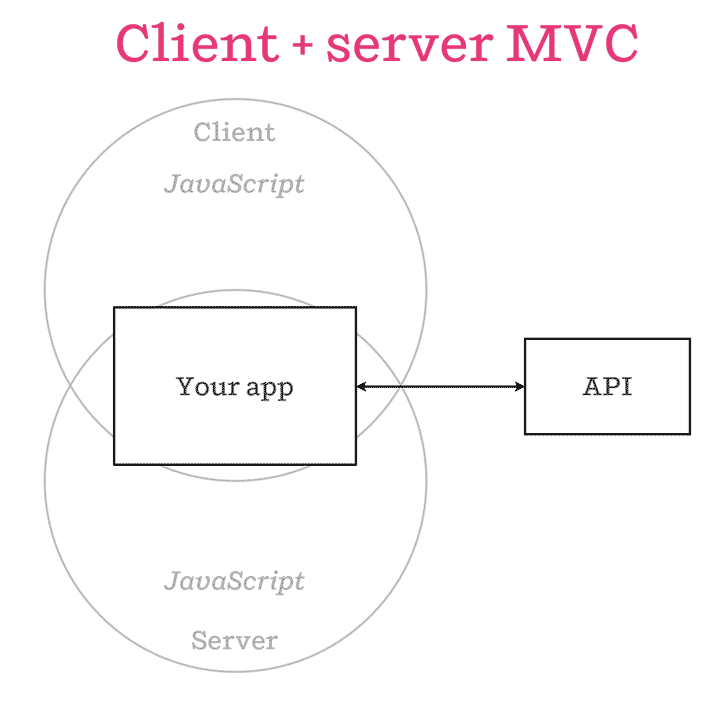
\includegraphics[width=0.5\textwidth]{figuras/estadoArte/isomorphic-client-server-mvc.png}
	\caption{\isomorphicAS  \clientAS \serverAS \mvcAS.}
	\label{figure:isomorphic_client_server_mvc}
\end{figure}

Algunas de las aplicaciones y \viewLogicAS que son utilizadas recurrentemente, pueden ser ejecutadas tanto en el \serverAS como en \clientAS. Esto permite nuevas posibilidades: \performanceQA \optimizationQA, mejor \maintainabilityQA, \seoINT por \defaultCPT, y más  aplicaciones \webINT \statefulINT.
%In this world, some of your application and view logic can be executed on both the server and the client. This opens up all sorts of doors — performance optimizations, better maintainability, SEO-by-default, and more stateful web apps.

Con la aparición de \nodejsNAME, un \fastQA, \stableQA \serverSideAS \javaScriptNAME \runtimeCPT, es factible hacer este sueño realidad. Creando las abstracciones apropiadas, es posible escribir \logicAS de aplicación que corra en el \serverAS y el \clientAS; justamente la definición de \isomorphicAS \javaScriptNAME.
%With Node.js, a fast, stable server-side JavaScript runtime, we can now make this dream a reality. By creating the appropriate abstractions, we can write our application logic such that it runs on both the server and the client — the definition of isomorphic JavaScript.

\subsection{\isomorphicAS \javaScriptNAME \frameworksPC}
\label{cap:justificacion:subsection:isomorphic_javaScript_framework}

\nodejitsuNAME escribió una gran descripción de una arquitectura \isomorphicAS \javaScriptNAME en 2011 \cite{online_nodejitsu_scaling_iso_js_code}, pero fue adoptado lentamente.
%This idea isn’t new — Nodejitsu wrote a great description of isomorphic JavaScript architecture in 2011 — but it’s been slow to adopt. There have been a few isomorphic frameworks to spring up already.

%Mojito was the first open-source isomorphic framework to get any press. It’s an advanced, full-stack Node.js-based framework, but its dependence on YUI and Yahoo!-specific quirks haven’t led to much popularity in the JavaScript community since they open sourced it in April 2012.

El \clientAS y el \serverAS son \environmentsPL muy distintos, y por lo tanto es necesario un conjunto de abstracciones que desacoplen la lógica de la aplicación desde su implementación subyacente, así se puede exponer una sola \apiAS para los desarrolladores.
%That these projects tend to be large, full-stack web frameworks speaks to the difficulty of the problem. The client and server are very dissimilar environments, and so we must create a set of abstractions that decouple our application logic from the underlying implementations, so we can expose a single API to the application developer.

\begin{itemize}
	\item
		\textbf{\routingAS}. Se desea un solo \setPL de \routesPC para \mapCPT patrones \uriNAME que \textit{manejar} \routePC. Los \handlersAS de \routePC necesitan disponibilidad de acceso a \httpNAME \headersINT, \cookiesINT, e información \uriNAME, y especificar redireccionamiento sin acceder directamente a \windowLocationINT(\browserINT) o \reqNodeINT y \resNodeINT (\nodejsNAME) \cite{online_isom_js_future_web_apps}.
		%Routing
		%We want a single set of routes that map URI patterns to route handlers. Our route handlers need to be able to access HTTP headers, cookies, and URI information, and specify redirects without directly accessing window.location (browser) or req and res (Node.js).
	\item
		\textbf{\fetchingPC y \persistingPC \dataPC}. Se desea describir los \resourcesCPT necesarios para \renderCPT una página particular o \componentAS independiente del mecanismo \fetchingPC \cite{online_isom_js_future_web_apps}.
		%El \resDescriptorCPT podría ser simplemente una \uriNAME apuntando a un \apiendpointAS \jsonNAME, o para aplicaciones largas, puede ser útil para \encapsulatePL \resourcesCPT en \modelsAS 
		%Fetching and persisting data
		%We want to describe the resources needed to render a particular page or component independently from the fetching mechanism. The resource descriptor could be a simple URI pointing to a JSON endpoint, or for larger applications, it may be useful to encapsulate resources in models and collections and specify a model class and primary key, which at some point would get translated to a URI.
	\item
		\textbf{\viewRenderingAS}. Ya sea que se decida manipular directamente \htmldomNAME, seguir con un \templatingAS \htmlNAME \stringBasePL, o bien optar como una de las \componentsAS \uiSiglaAS con una abstracción \htmldomNAME, es necesaria la capacidad de generar \markupPL \isomorphicallyAS. Es necesaria la factibilidad de \renderCPT cualquier \viewAS desde el \serverAS o el \clientAS, dependiendo solo de las necesidades de la aplicación \cite{online_isom_js_future_web_apps}.
		%View rendering
		%Whether we choose to directly manipulate the DOM, stick with string-based HTML templating, or opt for a UI component library with a DOM abstraction, we need to be able to generate markup isomorphically. We should be able to render any view on either the server or the client, dependent on the needs of our application.
	\item
		\textbf{\buildingPL y \packagingCPT}. Escribir código de aplicaciones \isomorphicAS es la mitad de la batalla. Herramientas como \grunttoolNAME y \browserifyNAME son partes esenciales del \workflowCPT para obtener una aplicación corriendo. Puede existir un número de \buildStepsPL: \compilingPL \templatesAS, incluyendo dependencias \clientSideAS, aplicando transformaciones, \minificationPL, etc. El caso sencillo es combinar todo el código de la aplicación, \viewsAS y \templatesAS en un único \bundleCPT, para aplicaciones grandes, esto puede resultar en cientos de \kilobytesPC para \downloadCPT. Un enfoque más avanzado es crear \dynamicBundlesCPT e introducir \lazyLoadingCPT \assetsAS, sin embargo, esto rápidamente se torna complicado. Herramientas \statAnalyCPT como \esprimaNAME permiten a desarrolladores ambiciosos intentar \optimizationQA y \metaprogrammingPC para reducir \boilerplateCodeAS.
		%Building and packaging
		%It turns out writing isomorphic application code is only half the battle. Tools like Grunt and Browserify are essential parts of the workflow to actually get the app up and running. There can be a number of build steps: compiling templates, including client-side dependencies, applying transforms, minification, etc. The simple case is to combine all application code, views and templates into a single bundle, but for larger apps, this can result in hundreds of kilobytes to download. A more advanced approach is to create dynamic bundles and introduce asset lazy-loading, however this quickly gets complicated. Static-analysis tools like Esprima can allow ambitious developers to attempt advanced optimization and metaprogramming to reduce boilerplate code.
\end{itemize}

Todo \frameworkPC que resuelve estos problemas al mismo tiempo es considerado un \isomorphicJSFwASref. Lo interesante de esto es que este tipo de \frameworksPC \textbf{permite a los desarrolladores enfocarse en la \businessLogicAS}.





%%%%%%%%%%%%%%%%%%%%%%%%%%%%%%%%%%%%%%%%%%%%%%%%%%%%%%%%%%%%%%%%%%%%%%%%%%%%%



%%%%%%%%%%%%%%%%%%%%%%%%%%%%%%%%%%%%%%%%%%%%%%%%%%%%%%%%%%%%%%%%%%%%%%%%%%%%%
%%%%%%%%%%%%%%%%%%%%%%%  	   METEOR FRAMEWORKS  	  %%%%%%%%%%%%%%%%%%%%%%%
%%%%%%%%%%%%%%%%%%%%%%%%%%%%%%%%%%%%%%%%%%%%%%%%%%%%%%%%%%%%%%%%%%%%%%%%%%%%%


\section{\meteorNAME}


\meteorNAME es un \environmentPL ultra-simple para construir \websitesINT modernos. Lo que antes demoraba semanas, incluso con las mejoras herramientas, ahora toma horas con \meteorNAME.
%Meteor is an ultra-simple environment for building modern websites. What once took weeks, even with the best tools, now takes hours with Meteor.

La \webINT fue diseñada originalmente para trabajar de la misma manera que los \mainframesAS funcionaban en los 70s. La aplicación del \serverAS \rendered una \screen y la envía a través de la \networkINT a un \dumbterminal (\refFigura{figure:mainframeServer_dumbterminal}). Si el usuario realizó alguna acción, el \serverAS \rendered una \screen completamente nueva. Este modelo funcionó bien para la \webINT por una década. Esto permitió la existencia de \lampNAME, \railsNAME, \djangoNAME, \phpNAME.
%The web was originally designed to work in the same way that mainframes worked in the 70s. The application server rendered a screen and sent it over the network to a dumb terminal. Whenever the user did anything, that server rerendered a whole new screen. This model served the Web well for over a decade. It gave rise to LAMP, Rails, Django, PHP.

\begin{figure}[h!]
	\centering
	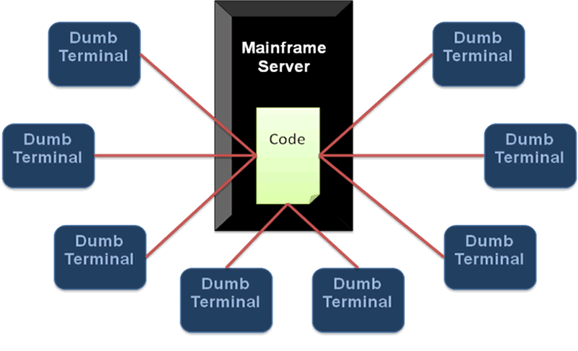
\includegraphics[width=0.6\textwidth]{figuras/mainframeServer_dumbterminal.png}
	\caption{Aquitectura de \mainframeAS con \dumbterminal}
	\label{figure:mainframeServer_dumbterminal}
\end{figure}


Pero los mejores equipos, con los mas grandes presupuestos y mas largos \schedules, ahora construyen aplicaciones en \javaScriptNAME que corren en el \clientAS. Estas aplicaciones tienen interfaces estelares. Estas aplicaciones no \reload \pages, son \reactive: cambios de cualquier \clientAS aparecen inmediatamente en las \screen de todos.
%But the best teams, with the biggest budgets and the longest schedules, now build applications in JavaScript that run on the client. These apps have stellar interfaces. They don't reload pages. They are reactive: changes from any client immediately appear on everyone's screen.

La aplicación fue construida de la manera difícil. \meteorNAME hace esto con la intención de ofrecer simpleza, y muchísima más entretención. Es posible construir una aplicación completa en un fin de semana, o en una \hackathonCPT con la suficiente cafeína. Ya no es necesario los \resourcesCPT del \serverAS, o \deploy \apiAS \apiendpointsAS en la \cloud, o manejar una \dataBaseDB, o desgastarse con una \orm \layerAS, o intercambiar \backandforth entre \javaScriptNAME y \rubyNAME, o \broadcast datos de invalidación a los \clientsAS.
%They've built them the hard way. Meteor makes it an order of magnitude simpler, and a lot more fun. You can build a complete application in a weekend, or a sufficiently caffeinated hackathon. No longer do you need to provision server resources, or deploy API endpoints in the cloud, or manage a database, or wrangle an ORM layer, or swap back and forth between JavaScript and Ruby, or broadcast data invalidations to clients.

\meteorNAME es un trabajo en desarrollo, pero se espera que muestra la dirección del equipo desarrollador. Ellos están deseosos de recibir \feedback. 
%Meteor is a work in progress, but we hope it shows the direction of our thinking. We'd love to hear your feedback.

\subsection{Principios de \meteorNAME}
%Principles of Meteor
\begin{itemize}
	\item \textbf{Datos \onthewire}. \meteorNAME no envía \htmlNAME a través de la \networkINT. El \serverAS envía datos y permite al \clientAS \renderCPT la información.
%Data on the Wire. Meteor doesn't send HTML over the network. The server sends data and lets the client render it.

	\item \textbf{Un lenguaje}. \meteorNAME permite escribir el código correspondiente al \clientAS y a el \serverAS de la aplicación en \javaScriptNAME.
%One Language. Meteor lets you write both the client and the server parts of your application in JavaScript.
	\item \textbf{\dataBaseDB en todas partes}. Se pueden utilizar los mismos métodos para acceder a la \dataBaseDB desde el \clientAS o el \serverAS.
%Database Everywhere. You can use the same methods to access your database from the client or the server.

	\item \textbf{Compensación de \latency}. En el \clientAS, \meteorNAME \prefetches datos y simula modelos para aparentar que los métodos del \serverAS retornan instantáneamente.
%Latency Compensation. On the client, Meteor prefetches data and simulates models to make it look like server method calls return instantly.

	\item \textbf{\fullstackAS \reactivity}. En \meteorNAME, \realTimeINT es el \defaultCPT. Todas las \layers, desde la \dataBaseDB hasta el \templateAS, \update por si mismo automáticamente cuando es necesario.
%Full Stack Reactivity. In Meteor, realtime is the default. All layers, from database to template, update themselves automatically when necessary.

	\item \textbf{\embraceecosystem}. \meteorNAME es un \openSourcePC e integra \toolsCPT y \frameworksPC \openSourcePC.
%Embrace the Ecosystem. Meteor is open source and integrates with existing open source tools and frameworks.

	\item \textbf{\simplicity igual \productivity}. La mejor manera para de hacer algo que parezca sencillo es tener lo que realmente sea simple. La principal funcionalidad de \meteorNAME tiene limpias y hermosas \apisAS clásicas.
%Simplicity Equals Productivity. The best way to make something seem simple is to have it actually be simple. Meteor's main functionality has clean, classically beautiful APIs.

\end{itemize}

\subsection{¿Qué es \meteorNAME?}
%What is Meteor?

\meteorNAME son dos cosas:
%Meteor is two things:
\begin{itemize}
	\item 
		Una librería de \packagesAS: \modulesAS \prewritten y \selfcontained que probablemente serán necesarios en las aplicaciones.
		%A library of packages: pre-written, self-contained modules that you might need in your app.

		Hay cerca de una docena de \packagesAS \coreAS \meteorNAME que prácticamente cualquier aplicación usará.  Dos ejemplos: \webapp, la cual \handleAS conexiones \incomming \httpNAME, y \templatingAS, lo que permite hacer \templatesAS \htmlNAME que automáticamente \update en vivo cuando los datos cambien. Entonces hay \packagesAS opcionales como \email, que permite a una aplicación enviar \emails, o la serie de cuentas de \meteorNAME las cuales proporcionan un sistema de cuentas de usuarios \fullFeatured que puede ser \droprightinto la aplicación. Adicionalmente a estos \packagesAS "\coreAS", hay miles de \packagesAS escritos por la comunidad, los cuales pueden ser necesarios para alguna aplicación propia.
		%There are about a dozen core Meteor packages that most any app will use. Two examples: webapp, which handles incoming HTTP connections, and templating, which lets you make HTML templates that automatically update live as data changes. Then there are optional packages like email, which lets your app send emails, or the Meteor Accounts series (accounts-password, accounts-facebook, accounts-ui, and others) which provide a full-featured user account system that you can drop right into your app. In addition to these "core" packages, there are thousands of community-written packages in Atmosphere, one of which might do just what you need.

	\item
		Una herramienta \commandLine llamada \commandLinemeteor.
		%A command-line tool called meteor.

		\commandLinemeteor es una herramienta de construcción análoga para hacer, examinar, o las partes no visuales de \visualstudio. Reúne todos los archivos y \assetsAS en la aplicación, lleva a cabo cualquier paso de construcción necesario (tal como compilar \coffeescript, \minifying \cssNAME, construir \modulesAS \npm, o generar \sourcemaps), trae los \packagesAS usados por la aplicación, y entrega un paquete independiente de aplicaciones \readytorun. En modo desarrollador puede hacer todo esto de manera interactiva, así que siempre que se cambie un archivo, inmediatamente se reflejaran los cambios en el \browserINT. Esto es muy sencillo utilizar \outofthebox, pero también es extensible: es posible agregar soporte para nuevos lenguajes y compiladores incluyendo \buildPL \pluginAS \packagesAS a la aplicación.
		%meteor is a build tool analogous to make, rake, or the non-visual parts of Visual Studio. It gathers up all of the source files and assets in your application, carries out any necessary build steps (such as compiling CoffeeScript, minifying CSS, building npm modules, or generating source maps), fetches the packages used by your app, and outputs a standalone, ready-to-run application bundle. In development mode it can do all of this interactively, so that whenever you change a file you immediately see the changes in your browser. It's super easy to use out of the box, but it's also extensible: you can add support for new languages and compilers by adding build plugin packages to your app.

\end{itemize}

La idea clave de \meteorNAME \packageAS \system es que todo debería funcionar exactamente igual en el \browserINT y en el \serverAS (siempre que esto tenga sentido, claramente \browsersINT no pueden enviar \emails y \serversAS no pueden capturar eventos del \mouse). El ecosistema completo ha sido construido desde cero para soportar esto.
%The key idea in the Meteor package system is that everything should work identically in the browser and on the server (wherever it makes sense, of course: browsers can't send email and servers can't capture mouse events). Our whole ecosystem has been built from the ground up to support this.

\subsection{El \stackAS \meteorNAME}


El \stackAS \meteorNAME(\refFigura{figure:meteor_stack}) es un miembro de la familia \meanstackNAME, esto significa que esta impulsado por \nodejsNAME en el \serverSideAS. Es el mismo propósito que tiene el \webserverINT \apacheNAME en el \stackAS \lampNAME.



\begin{figure}[h!]
	\centering
	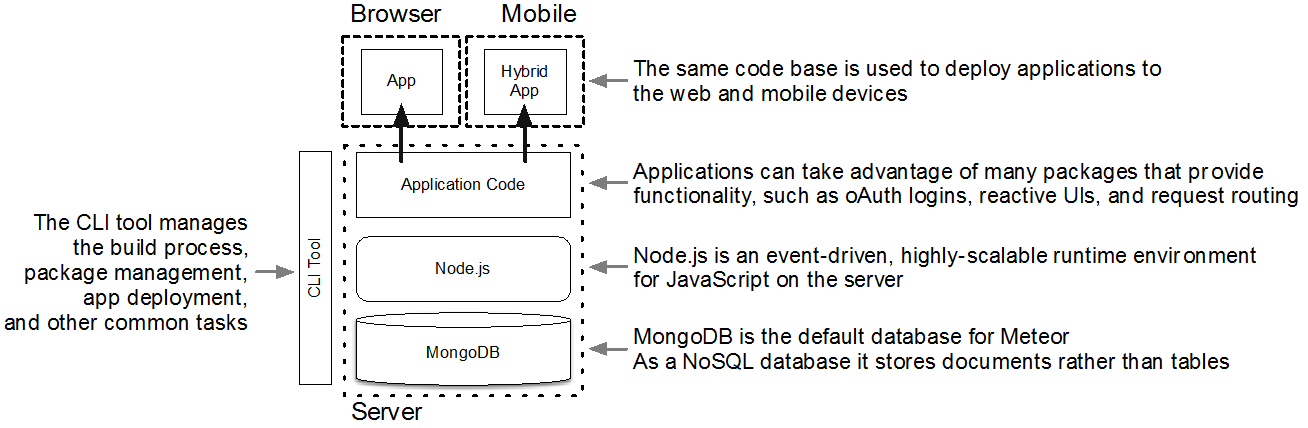
\includegraphics[width=1.0\textwidth]{figuras/meteor_stack.png}
	\caption{El \stackAS \meteorNAME corre aplicaciones potenciadas por \packagesAS inteligentes sobre \nodejsNAME y \mongodbNAME}
	\label{figure:meteor_stack}
\end{figure}

Toda la información es típicamente guardada dentro de \mongodbNAME. Provee una \apiAS \javaScriptNAME que da acceso a todo el contenido almacenado en forma de \documentsDB ó \objectsPL. El mismo lenguaje dentro del \browserINT puede ser usado para acceder a los datos, el cual \meteorNAME toma ventaja para implementar un verdadero desarrollo \fullstackAS.
%All data is typically stored inside a MongoDB, a document-oriented NoSQL database. There are plans for Meteor to support other (SQL-based) database systems, but currently the only suggested DB is Mongo. It provides a JavaScript-API that gives access to all stored content in form of documents or objects. The same language used inside the browser can be used to access data, which Meteor takes advantage to implement true fullstack development.

Todo el \softwarePC y librerías requeridas para crear aplicaciones \webINT desde cero son agrupados en forma de \packagesAS inteligentes, así los desarrolladores pueden empezar de inmediato. Estos \packagesAS incluyen una librería de interfaz de usuario (\blazemeteor), un manejador de cuentas de usuarios (\accountsmeteor), y mantener a todos los \clientsAS \reactively \updated en \realTimeINT (\trackermeteor).
%All required software and libraries required to create web applications from scratch are bundled in the shape of Smart Packages, so developers can get started right away. These packages include a user interface library (Blaze), managing user accounts (accounts), and keeping all clients reactively updated in realtime (Tracker).

La herramienta \clitool de \meteorNAME permite a los desarrolladores rápidamente \setupCPT un \environmentPL completo de desarrollo. No es necesario saber como instalar o configurar algún \softwarePC de \serverAS. \meteorNAME cuida literalmente los aspectos de la infraestructura. Esto es también una herramienta para construir, comparable a \maketool ó \grunttoolNAME, y un manejador de \packageAS, tal como \apttool ó \npm. Finalmente la herramienta \clitool agrupa una aplicación para correr en diferentes plataformas de \clientsAS, dentro de un \browserINT \webINT ó como una aplicación \mobileINT nativa.
%The Meteor CLI tool allows developers to quickly set up an entire development environment. There is no need to know how to install or configure any server software, Meteor takes care of the infrastructure aspect entirely. It is also both a build tool, comparable to make or grunt, and a package manager, such as apt or npm. For example it can compile LESS or CoffeeScript on the fly, without first setting up workflow or add authentication via Facebook oAuth with a single command. Finally the CLI tool bundles an application to run on different client platforms, inside a web browser or as native mobile apps.

Todas las partes del \stackAS se integran sin problemas, todos los \packagesAS \coreAS son diseñados y probados para trabajar bien en conjunto. Por otro lado, es perfectamente posible cambiar partes del \stackAS a otros, en caso de ser necesario. En lugar de utilizar \meteorNAME en su totalidad podría decidir utilizarse sólo los componentes de \serverAS y utilizar por ejemplo \angularjsNAME para el \clientSideAS, o utilizar un \javabackend que utilice \meteorNAME en el \frontEndAS para proveer \updates \realTimeINT para todos los \clientsAS.
%All parts of the stack integrate seamlessly, all core packages are designed and tested to work well together. On the other hand, it is entirely possible to switch out parts of the stack for others, should the need arise. Instead of using Meteor in full you could decide to only use the server components and use e.g. Angular.js on the client side, or use a Java-backend that uses Meteor on the front-end to provide realtime updates to all clients. 

\subsection{\frameworkPC \isomorphicAS – \fullstackAS \javaScriptNAME}
%Isomorphic Frameworks – Fullstack JavaScript

\meteorNAME corre sobre \nodejsNAME y mueve la lógica de la aplicación hacia el \browserINT, lo que es usualmente referido a \singlePageAppINT. El mismo lenguaje es usado sobre todo el \stackAS, lo que transforma a \meteorNAME en una plataforma \isomorphicAS. Como resultado el mismo código \javaScriptNAME puede ser usado en el \serverAS, en el \clientAS, e incluso en la \dataBaseDB.
%Meteor runs on top of Node.js and moves the application logic to the browser, which is often referred to as Single Page Applications. The same language is used across the entire stack, which makes Meteor an isomorphic platform. As a result the same JavaScript code can be used on the server, the client, and even in the database. 

Mientras muchos \frameworksPC usan el mismo lenguaje en tanto en \clientAS como en \serverAS, la mayoría del tiempo estos no pueden compartir código porque los \frameworksPC no son íntimamente integrados, por ejemplo el uso de \angularjsNAME en el \frontEndAS y \expressjsNAME en el \backendAS. \meteorNAME es un \fullstackAS verdadero porque usa una simple y unificada \apiAS expuesta para todas las funcionalidades \coreAS y pueden ser utilizadas en el \serverAS, en el \browserINT, e incluso para acceder a la \dataBaseDB. Para comenzar, no es necesario aprender múltiples \frameworksPC y da como resultado una mejor \reusabilityQA del código solo utilizando el mismo lenguaje.
%While many frameworks use the same language on both client and server, most of the times they cannot share code between the two instances because the frameworks are not tightly integrated, for example they use Angular on the frontend and Express.js on the backend. Meteor is truly fullstack because it uses a simple and unified API that exposes all core functionality and can be used on the server, in the browser, and even to access the database. To get started you do not have to learn multiple frameworks and results in much better re-usability of the code than only using the same language.

Para acceder a la \dataBaseDB desde el \browserINT, \meteorNAME incluye una mini \dataBaseDB. Esta simula exactamente la misma \apiAS de una \dataBaseDB. Dentro del \browserINT \minimongo permite a los desarrolladores utilizar los mismos comandos como si estuvieran en una consola de \mongodbNAME.
%To access the database from the browser, Meteor includes mini  databases. They simulate the exact same API of a database. Inside the browser Minimongo allows developers to use the same commands as they would in a MongoDB console.

Típicamente los desarrolladores necesitan saber como escribir código que tome una completa ventaja del \eventloopCPT y que funciones corren \synchronously y cuales \asynchronously (\nameref{cap:section:nodejs}). Mientras mas funcionalidades \asynchronously son utilizadas, tanto mayor serán los \callbacksPL envueltos y las cosas se vuelven bastante sucias.
%Typically, developers need to know how to write code that takes full advantage of the event loop and what functions run synchronously and which asynchronously. The more asynchronous functionality is used, the more callbacks are involved and things can become quite messy.

Afortunadamente, \meteorNAME aprovecha toda la potencia de \eventloopCPT, pero facilita el proceso evitando cierta preocupación sobre escribir código \asynchronousCPT. Utiliza el concepto llamado \fibers \behindthescenes. \fibers proveen una capa de abstracción para el \eventloopCPT que ejecuta funciones \asynchronousCPT(\tasks) en secuencia. Esto elimina la necesidad de \callbacksPL explícitos de manera que se puedan utilizar un estilo \synchronousCPT familiar.
%Fortunately, Meteor leverages the full power of the event loop, but it makes it easy by not having to worry so much about writing asynchronous code. It uses a concept called Fibers behind the scenes. Fibers provide an abstraction layer for the Event Loop that executes asynchronous functions (tasks) in sequence.It removes the need for explicit callbacks so that a familiar synchronous style may be used.

\subsection{¿Por qué \meteorNAME?}

No importa lo bueno que una aplicación sea, la cantidad de prestaciones, en fin....  Incluso puede ser superior a las que los competidores presentan; todo esto significa nada si finalmente la aplicación no es utilizada por los usuarios objetivos.

Esta misma afirmación se aplica para el caso de los \frameworksPC; no importa cuan interesante pueda ser, cuantas \toolsCPT provee, etc; si no existe una comunidad activa creando nuevo contenido, solucionando infinidad de problemas, incluso encontrando \bugsPL para lograr una versión más estable. O lo que es lo mismo, si existe una gran comunidad activa, entonces tienes un \frameworkPC con un gran respaldo.

\hotframeworksNAME es un \websiteINT que se dedica a posicionar los \frameworksPC en un \rankingCPT de acuerdo a lo popular que estos sean, o lo que es lo mismo, de acuerdo a cuan activa es su comunidad. Dicho estudio, que se aprecia en \reftabla{tab:position_meteor_global_ranking_framework}, posiciona a \meteorNAME en la sexta posición.

%%%%%%%%%%%%%%%%%%%%%%%%%%%%%%%%%%%%%%%%%%%%%%%%%%%%%%%%%%%%%%%%%%%%%%%%%%%%%
%%%%%%%%%%%%%%%%%%%  	   TABLE RANKING FRAMEWORKS  	  %%%%%%%%%%%%%%%%%%%
%%%%%%%%%%%%%%%%%%%%%%%%%%%%%%%%%%%%%%%%%%%%%%%%%%%%%%%%%%%%%%%%%%%%%%%%%%%%%

\begin{table}[h!]
    \center
 
\begin{tabular}{ |c|c|c|c| }
\hline
	\frameworkPC &
	\gitHubNAME \scoreCPT&
	\stackOverflowNAME \scoreCPT &
	\overallScoreCPT
 
\\ \hline
	\aspNetNAME&
	-&
	100&
	100
	
\\ \hline
	\rubyonrailsNAME&
	96&
	98&
	97

\\ \hline
	\angularjsNAME&
	100&
	90&
	95

\\ \hline
	\aspNetMvcNAME&
	-&
	93&
	93

\\ \hline
	\djangoNAME&
	89&
	91&
	90

\\ \hline
	\meteorNAME&
	95&
	74&
	84
	

\\ \hline
\end{tabular}
    \caption{ Ubicación del \frameworkPC \meteorNAME \cite{online_hotframeworks_official_site}}
    \label{tab:position_meteor_global_ranking_framework}
\end{table}

%%%%%%%%%%%%%%%%%%%%%%%%%%%%%%%%%%%%%%%%%%%%%%%%%%%%%%%%%%%%%%%%%%%%%%%%%%%%%

Importante recordar que este \rankingCPT incluye todos los \frameworksPC sin discriminar. Entonces, no solo es el sexto \frameworkPC con la mayor comunidad activa, si no que es el primer solo considerando los \frameworkPC \javaScriptNAME \isomorphicAS.

\subsection{ ¿Por qué son necesarios los \frameworksPC?}
% [http://www.codeproject.com/Articles/5381/What-Is-A-Framework]

Un \frameworkPC es un conjunto de bloques de \softwarePC comunes y prefabricados que los programadores pueden utilizar, extender o customizar para soluciones específicas. Con  \frameworksPC los desarrolladores no necesitan comenzar a escribir una aplicación en cada oportunidad desde el principio. \frameworksPC son construidos desde una colección de objetos tal que tanto el diseño como el código del \frameworkPC pueden ser reutilizados \cite{online_frontier_what_is_framework}.
%A framework is a set of common and prefabricated software building blocks that programmers can use, extend or customize for specific computing solutions. With frameworks developers do not have to start from scratch each time they write an application. Frameworks are built from collection of objects so both the design and code of the framework may be reused. - JavaFramework.

Un esqueleto de una aplicación en la cual los desarrolladores \plugAS en sus códigos y proveen la mayoría de las funcionalidades comunes \cite{book_addisonwesley_what_is_framework}.
%A skeleton of an application into which developers plug in their code and provides most of the common functionality.  -- E. Gamma, et al., "Design Patterns", Addison-Wesley, 1995

%***************************************************************************
%Well, now that's a radically different definition, and in my thinking certainly incorporates the idea of a methodology, if for no other reason than because the "skeleton" has to define how developers plug in their code and how they interface with the common functionality provided by the "skeleton".  Implied here (but not necessarily) may also be how the code intercommunicates.
%
%A set of classes which defines a model of interaction among objects… -- Moduleco (of course, they totally blow it in the additional definitions)
%
%OK, this falls into the category of a methodology because it clearly enforces the interaction style between objects, but it leaves out the wrapper and architectural aspects.
%
%A comprehensive, integrated class library
%An entire architecture is the unit of reuse
%Defines the control logic and class interactions of the application's architecture
%Reduces "dog work" at the cost of some flexibility
%-- Software Engineering Associates, Inc
%***************************************************************************


Un \frameworkPC es un directorio con jerarquía que encapsula recursos compartidos, tales como, \dynamSharedLibAS, documentación de referencia, imágenes, en un solo \packageAS. Múltiples aplicaciones pueden utilizar todos los recursos de manera simultanea. El sistema los carga en \memoryPC según necesidad y comparte una copia de los recursos entre todas las aplicaciones posibles \cite{online_apple_what_is_framework}.
%A framework is a hierarchical directory that encapsulates shared resources, such as a dynamic shared library, nib files, image files, localized strings, header files, and reference documentation in a single package. Multiple applications can use all of these resources simultaneously. The system loads them into memory as needed and shares the one copy of the resource among all applications whenever possible.

De acá se difiere que no existe una definición única para lo que significa el concepto \frameworkPC. Sin embargo, todo \frameworkPC debería ser simultáneamente: 

\begin{itemize}
	\item \textbf{Un \wrapperAS} es una manera de \repackagingAS una función ó un conjunto de funciones(no necesariamente relacionadas) para lograr al menos uno de los siguientes objetivos: Simplificar uso; Consistencia en Interfaz; Mejora de las funcionalidades \coreAS; Recolectar procesos discretos dentro de una asociación lógica(un \objectPL) \cite{online_codeProject_what_is_framework}.

		\begin{figure}[H]
			\centering
			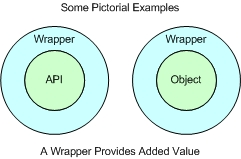
\includegraphics[width=0.4\textwidth]{figuras/framework_component_wrapper.jpg}
			\caption{Un \wrapperAS provee valor agregado.}
			\label{figure:framework_component_wrapper}
		\end{figure}

	\item \textbf{Una \architectureCPT} es un estilo que incorpora elementos de diseño específicos \cite{online_codeProject_what_is_framework}.

		\begin{figure}[H]
			\centering
			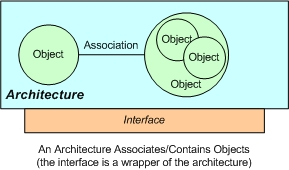
\includegraphics[width=0.4\textwidth]{figuras/framework_component_architecture.jpg}
			\caption{Una \architectureCPT \asociatesAS/\containsAS \objectsPL. (La \interfaceAS es un \wrapperAS de la \architectureCPT.)}
			\label{figure:framework_component_architecture}
		\end{figure}

	\item \textbf{\methodologyCPT} Es la manera para realizar algo. En este caso, define las interacciones entre \architectureCPT, \componentsAS y \objectsPL \cite{online_codeProject_what_is_framework}.

		\begin{figure}[H]
			\centering
			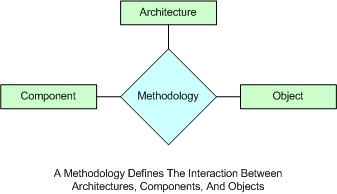
\includegraphics[width=0.4\textwidth]{figuras/framework_component_methodology.jpg}
			\caption{Una \methodologyCPT define las interacciónes entre \architectureCPT, \componentsAS y \objectsPL.}
			\label{figure:framework_component_methodology}
		\end{figure}

\end{itemize}

Elegir el \frameworkPC correcto para un proyecto puede tener un impacto tremendo en la habilidad de entregar a tiempo y la habilidad para mantener el código en el futuro. ES ciertamente deseable un \frameworkPC sólido, estable y probado, pero sin estar limitado por la opción.

%%%%%%%%%%%%%%%%%%%%%%%%%%%%%%%%%%%%%%%%%%%%%%%%%%%%%%%%%%%%%%%%%%%%%%%%%%%%%